\chapter{A Visualization Interface for Efficient Simulation Uncertainty Analysis}
\section{Introduction: Uncertainty Analysis for Simulations}
Almost all scientific research using simulations shares certain goals. To test hypotheses and predict outcomes, scientists must understand how initial conditions and parameterizations affect observable quantities, their uncertainties, and their agreement with experimental data. Visualization software tools have been used to analyze simulations in a wide breadth of domains for decades. However, understanding uncertainty in simulation data, a task vital to the scientific process, is particularly difficult with conventional visualization tools \cite{bonneau}.

The necessary software, which would facilitate rapid, dynamic exploration of uncertainty, is difficult to design. Uncertainty in large simulations is complex, with intertwined causes and effects. Sources of uncertainty include unknown input conditions, unknown external factors, internal variability due to complex physical processes, and differences in the algorithmic formulations of these processes \cite{Deser2012}, \cite{georgakakos}, \cite{haroz:2008}. Experimental data providing the ground truth for simulations are also uncertain for a variety of reasons~\cite{gleckler}.

Uncertainty from discretization, or ``discreteness noise''~\cite{rau}, affects all simulations. When continuous physical properties, such as temperatures or mass distributions, are modeled with the discretized equations necessary for computer simulations, and sampled in discrete bins or timesteps, the system being modeled is inherently misrepresented, and measurements of its output are uncertain. 
% note: make clearer that 'discretization uncertainty' is part of the larger category of 'model uncertainty' -- this is how most papers talk about it

%note: one of our goals is to let scientists explore the parameter spaces of their simulations

This ``discreteness noise'' can be measured by applying bootstrapping, a statistical technique for sampling data, and measuring the variance in the bootstrapped samples~\cite{rau},~\cite{vavrus}. (Modifications to address problems with bootstrapping have been proposed, e.g.,~\cite{Steck}; they can be substituted in our work as desired.) For large simulations, measuring discreteness noise this way takes a long time and must be re-performed in the case of new initial conditions or parameters. 

To measure discreteness noise more quickly and flexibly, we propose a visualization tool to facilitate bootstrapping small subsamples of simulation data, identifying patterns in these samples, then helping train regression models of the uncertainty in the original data (Figure~\ref{workflow}). Visual exploration is key at each step of this process to understand patterns and ensure accurate modeling. In order to model and predict the uncertainty in the source dataset using subsamples, an algorithm must extrapolate patterns that exist in measurements of the samples. In general, humans are much better at pattern extrapolation tasks than algorithms are~\cite{HumanKernel}; extrapolation is difficult for regression models to perform. Human-aided methods, like the one we propose, can leverage the power of regression models enhanced by human pattern recognition and domain expertise.
%NOTE: need to be more precise here about where exactly machines/humans are strong/weak, and why we are using regression at all %

More specifically, regression models depend on kernels, which are functions determining how a model samples input data, and on scaling of those data. Kernels are specified by several parameters; extrapolation in particular, while possible with the correct regression methods, is highly sensitive to these parameters~\cite{WilsonGCN14}. Without understanding the kernel creation process, the relationship between the data's properties and the appropriate feature scaling is opaque to users. With a well-designed visualization tool, we can provide enough information for users to identify qualities of their data and guide a regression algorithm to predict uncertainty for their specific use case.

We evaluate our tool through case studies on simulations in three distinct domains (cosmology, traffic, and oceans), comparing our results with the ground truth, as well as through interviews with scientists. We envision several possible uses. Scientists can view patterns in the uncertainty in measurements of the subsamples, which may reveal effects of discreteness noise, and they can examine predicted uncertainty for the full dataset, changing input parameters as needed by feeding them into already-trained models.

\begin{figure}[h]
    \centering
    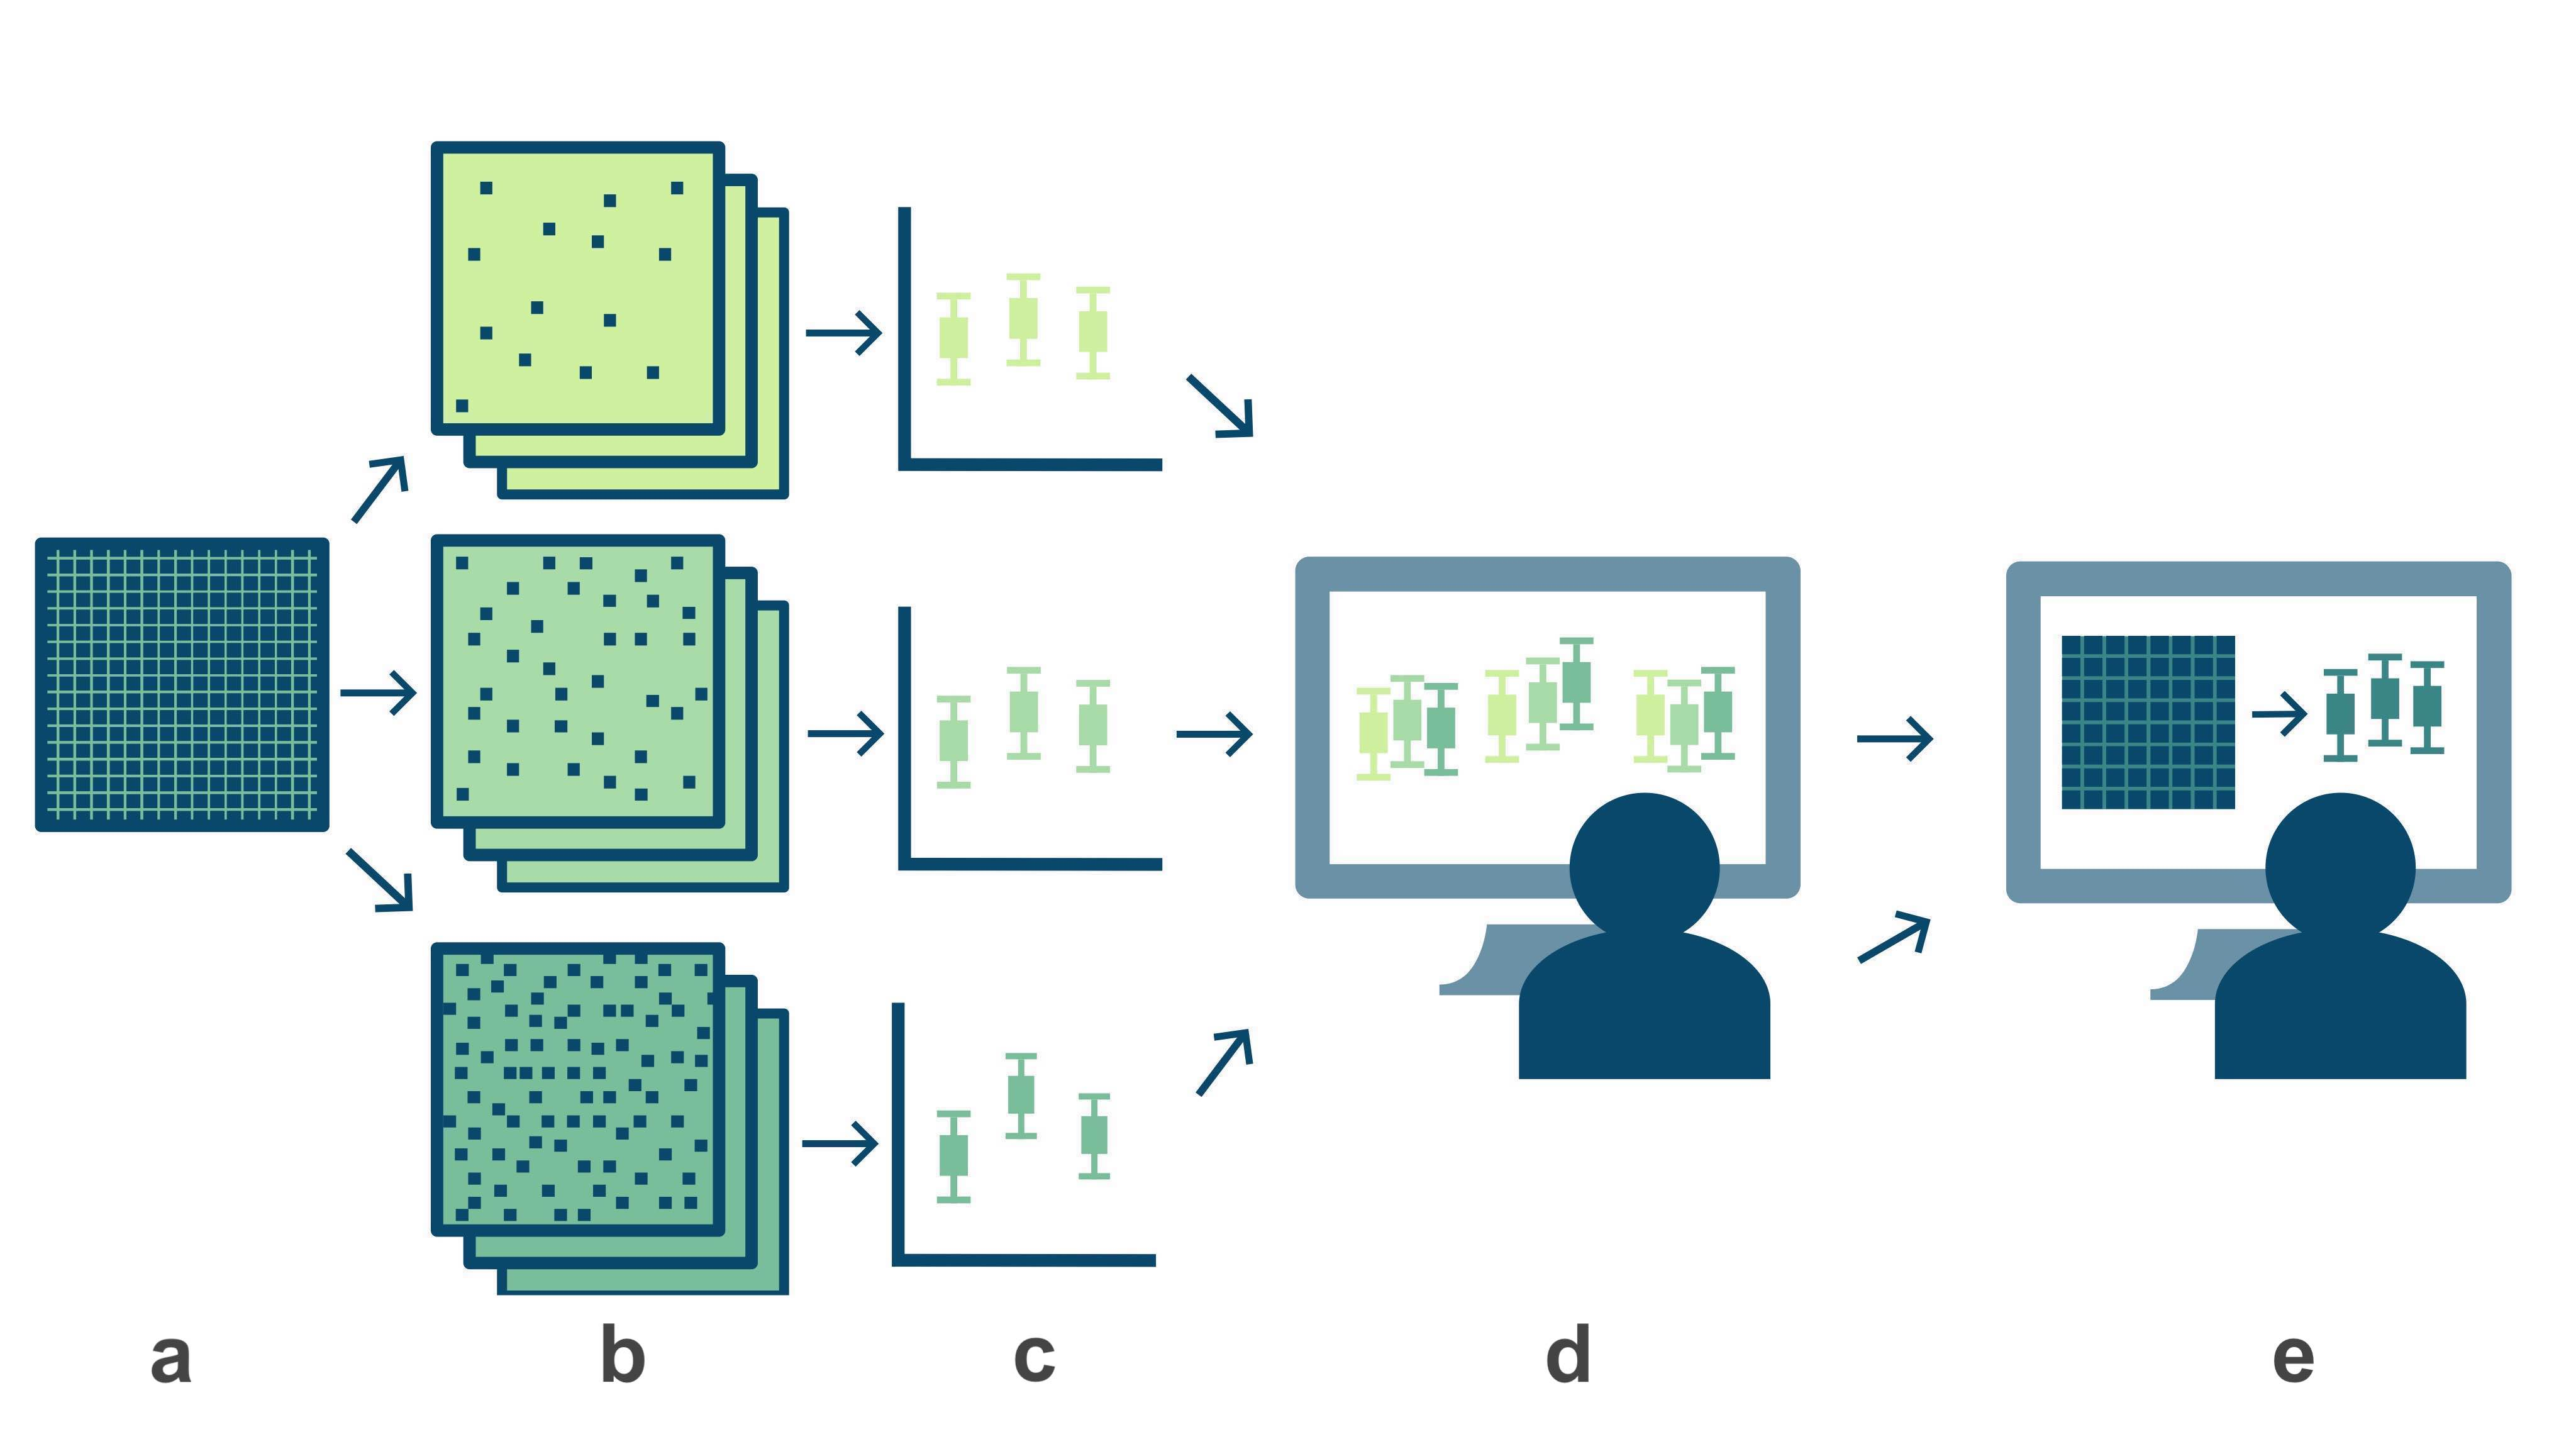
\includegraphics[width=\textwidth]{images/sampling/uncertainty_with_small_samples_labeled}
    \caption{Our proposed workflow. From the full dataset (a), a user extracts small random samples, then performs bootstrapping to extract an array of samples for each size (b). A measurement is performed on these samples, yielding estimates of uncertainty in this measurement (c). The user can inspect these uncertainties and identify patterns (d), then use their judgment to supervise training of a model that predicts the uncertainty on the full dataset (e). %(NOTE: need to reference in text.)
    }
     \label{workflow}
\end{figure}

Our contributions include:
\begin{itemize}
\item{A novel technique for efficiently estimating ``discreteness noise'' and its effect on simulation analysis.}
\item{An examination of how sample-based uncertainty prediction can be applied to simulation analysis in several fields.}
\item{A visual interface for user-supervised uncertainty prediction.}
\end{itemize}

\section{Background and Related Work}
We introduce the simulations we will use for testing and their underlying uncertainty. First, we discuss existing research related to uncertainty visualization, visual interfaces for machine learning, and simulation uncertainty quantification.

\subsection{Related Work}
Uncertainty is often identified as one of the most important challenges in visualization~\cite{curveboxplot}. There are several thorough overviews of the state of uncertainty visualization, such as~\cite{bonneau}. These summaries highlight a neglect for uncertainty in visualization research; many approaches have been proposed, but uncertainty is generally excluded from visualizations and is often seen as an afterthought, though it is crucial for scientific analysis. More work has focused on visual representations of uncertainty than on elucidating sources of uncertainty with visualization, and in particular, quantifying and modeling uncertainty is difficult and has been neglected~\cite{bonneau}.
%(cite referenced sources for this; use their related work section for a lot of sources) 
Visualizations of uncertainty must be enabled by robust quantitative analysis, which is often highly domain-specific. Here, we describe existing work in visualizing uncertainty and quantifying it for visualization.

\subsubsection{Uncertainty Visualization}
Some uncertainty work has been done from the perspective of visual analytics: tasks like data gathering, manipulation, visualization, and user perception all introduce uncertainties that users need to understand in order to properly draw conclusions from data \cite{sacha}. Researchers have created uncertainty-aware visual analytics frameworks, such as node-link diagrams enhanced with glyphs indicating uncertainty \cite{liu}. To visualize uncertainty propagation through a series of data transformations, the authors of \cite{correa2009framework} use Gaussian mixture models to model ``aggregated uncertainty'' from these transformations, enabling visualizations that show the variability in derived data with scatter plots and covariance matrices. The authors of \cite{wu} expand on this work, adding ellipsoids representing covariance for particular variables and flow trees to show the relative uncertainty introduced with each data transformation choice. 

There are many visual metaphors for uncertainty that compound on standard approaches such as boxplots and standard deviation curves. The authors of~\cite{contourboxplot} and~\cite{curveboxplot} introduce a boxplot-based visualization approach, and underlying statistical calculation, for understanding uncertainty in ensembles of curves or paths. Other modifications to standard boxplots have been proposed, such as ``functional boxplots''~\cite{functionalboxplots}, which use curves to enhance users' understanding of a data distribution and its outliers, and ``beanplots''~\cite{beanplot}, which additionally indicate the number of measurements in a sample. Uncertainty can be visualized using blurring effects \cite{haroz:seeing}. Visualizing uncertainty in physical space, such as in bounded 3-dimensional volumes, is challenging, as it can occlude other variables, and users are not used to seeing uncertainty depicted in three dimensions as they are in two \cite{haroz:2008}, \cite{li}. Color can also indicate uncertainty \cite{potter:2009}, especially in 3D space, or ``cones'' showing possible trajectories \cite{li}; the authors also employ ``magic glasses,'' allowing users to show or hide uncertainty information on top of the original data. These techniques may be more useful for expressing qualitative properties of data uncertainty than for precise quantitative analysis.

Uncertainty in scientific data, which are often multidimensional and require precise quantitative understanding, compounds on the challenges in uncertainty visualization. Simulation uncertainty is commonly analyzed by considering the results from an ensemble of simulation runs, perhaps with slightly perturbed initial conditions. The authors of \cite{potter:2009} use a variety of methods for visualizing this uncertainty in a climate model ensemble, using both spatial views (color on a map indicating standard deviation in that location; contours indicating probability levels; spaghetti plots of possible trajectories) and two-dimensional views (quartile trend charts; plume trend charts). Spaghetti plots can also be combined with glyphs representing uncertainty, and these plots can also be reimagined as graduated ribbons as in \cite{sanyal}. However, most climate ensembles do not use enough models to support such nuanced characterizations of their underlying uncertainty \cite{potter:2009}.

\subsubsection{Uncertainty Modeling}
Some nonparametric methods, which can capture outliers and noise better than parametric modeling of uncertainty can, exist, but require very fine parameter tuning~\cite{curveboxplot}. Quantitatively modeling uncertainty in physical data, such as those from scientific simulations, introduces more challenges. For example, temporal downsampling introduces uncertainty to values that are interpolated across timesteps. To address uncertainty in particle paths arising from interpolation between downsampled time steps, the authors of \cite{chen2015uncertainty} developed a polynomial-based error modeling method, using Bezier curve fitting to reconstruct physically plausible paths and visualize the results. Categorization of features, such as vortices, in simulations is often a binary choice, meaning that including uncertainty information in these classifications is difficult. The authors of \cite{biswas2015uncertainty} use fuzzy inputs and a consensus-based visualization tool to improve vortex classification in simulations.

A possible approach to modeling uncertainty from a simulation is to train a Gaussian process emulator to model a simulation using only its most influential input parameters, allowing rapid prediction of uncertainty \cite{gomez2014dissecting}. One can also use Bayesian Model Averaging to visualize the predictive uncertainty of model ensembles and individual models, as in~\cite{gosink}. Instead of calculating uncertainties and visualizing the result, representative sampling can be used to display uncertainty information to avoid occlusion while maintaining statistical properties \cite{liu2017uncertainty}. The authors of~\cite{doi:10.1029/2008WR006839} introduce a machine learning-based method for estimating uncertainty by learning the relationship between the distributions of input variables and model errors. It performs well at measuring uncertainty in a specific hydrological model, but is not capable of extrapolation, meaning that training examples must span the range of possible input variables.

%machine learning feature visualization

%specifically: ensemble visualization, flow visualization, 

%The unsupervised clustering visualization in~\cite{kwon_clustervision_2018} includes visualization of feature value distributions. (...)
\subsection{Data}
\label{data}

We use three simulations to test our uncertainty modeling method. We chose these datasets in order to highlight that our method can address different sources of uncertainty. For each simulation type, we identify a testing/training dataset and a calculation of interest. These simulations, depicted in Figure~\ref{data_examples}, have differing properties representative of the range of simulations that scientists use.


\begin{figure*}[h]
    \centering
    \begin{subfigure}{0.31\textwidth}
        \fbox{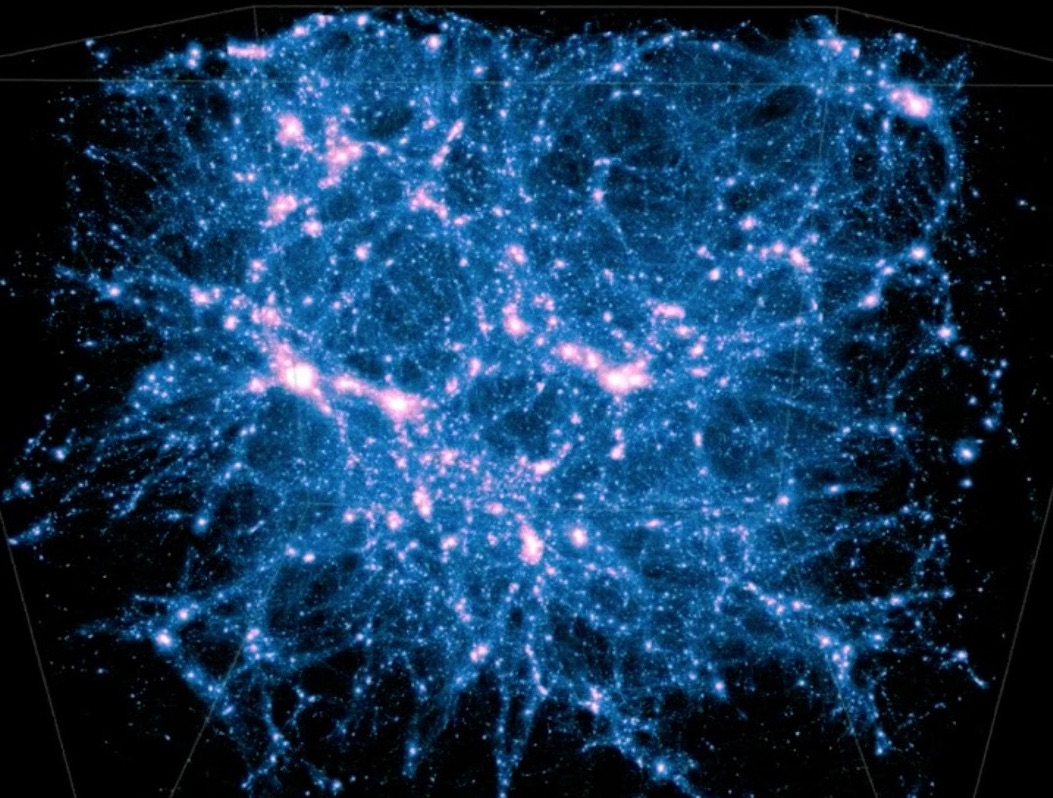
\includegraphics[width=\textwidth]{images/sampling/illustris_screenshot.jpg}}
        \caption{}
        \label{illustris_example}
    \end{subfigure}
    \begin{subfigure}{0.32\textwidth}
        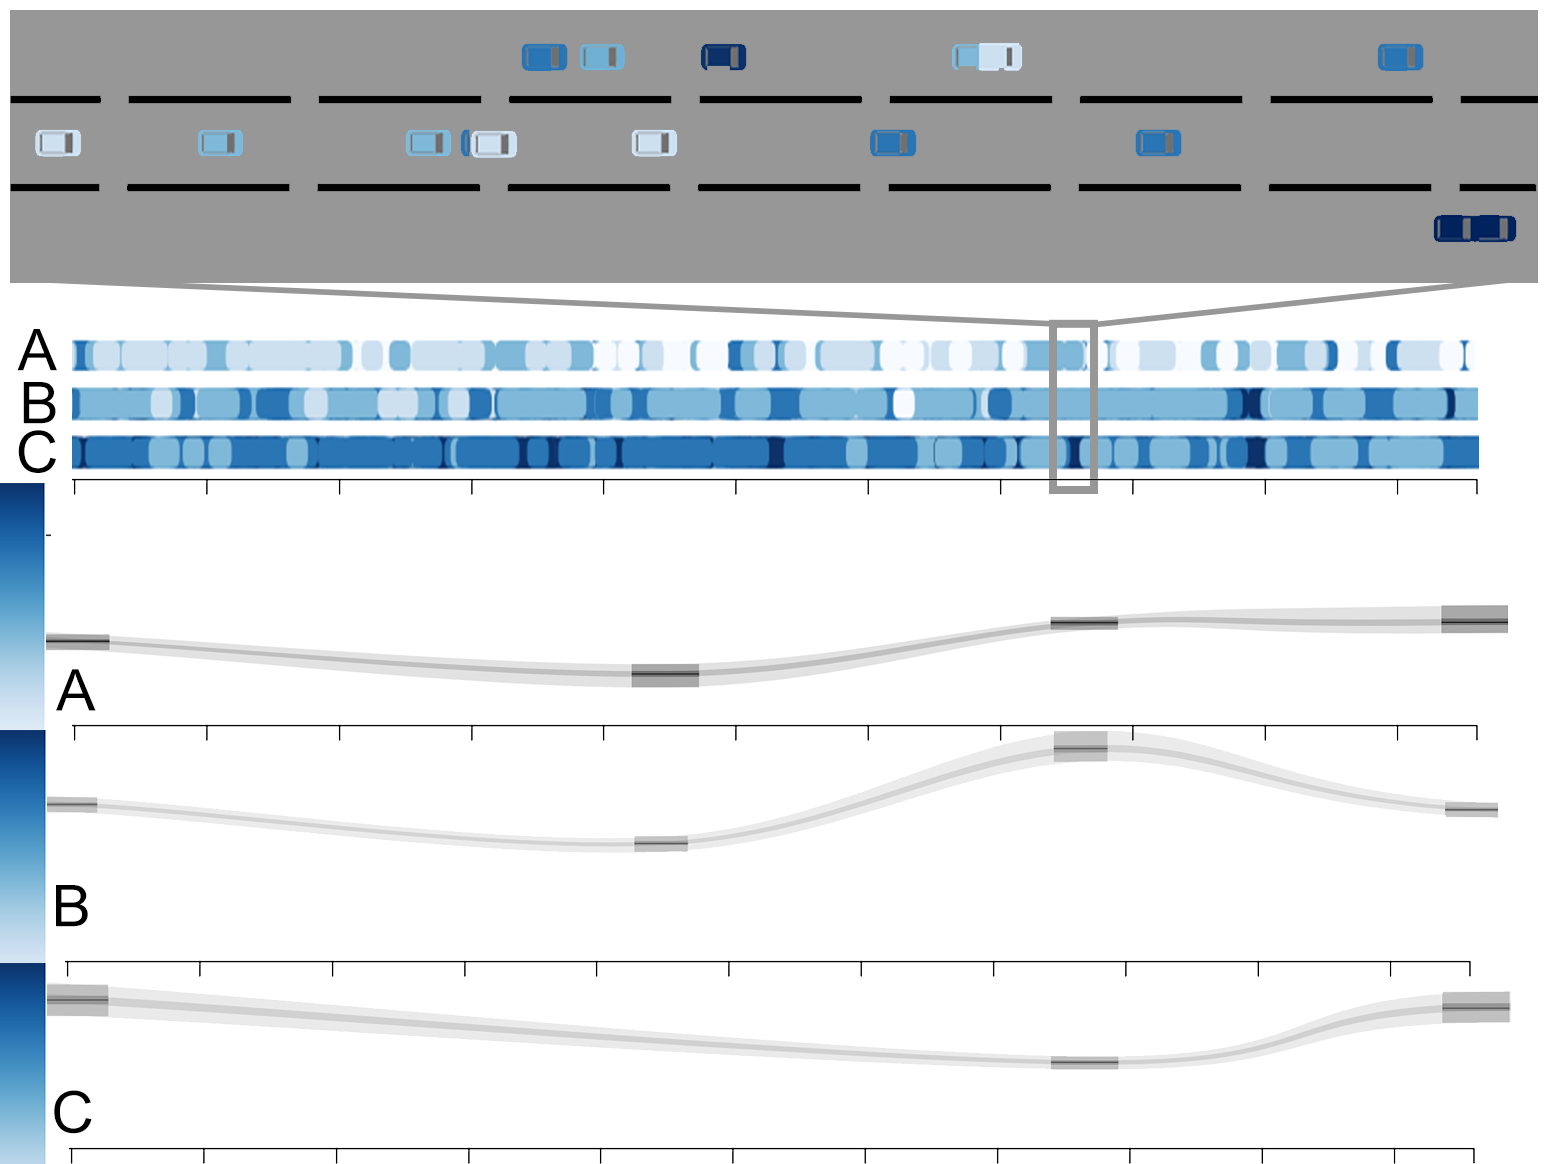
\includegraphics[width=\textwidth]{images/sampling/traffic_example_updated.png}
        \caption{}
        \label{sumo_example}
    \end{subfigure}
    \begin{subfigure}{0.32\textwidth}
        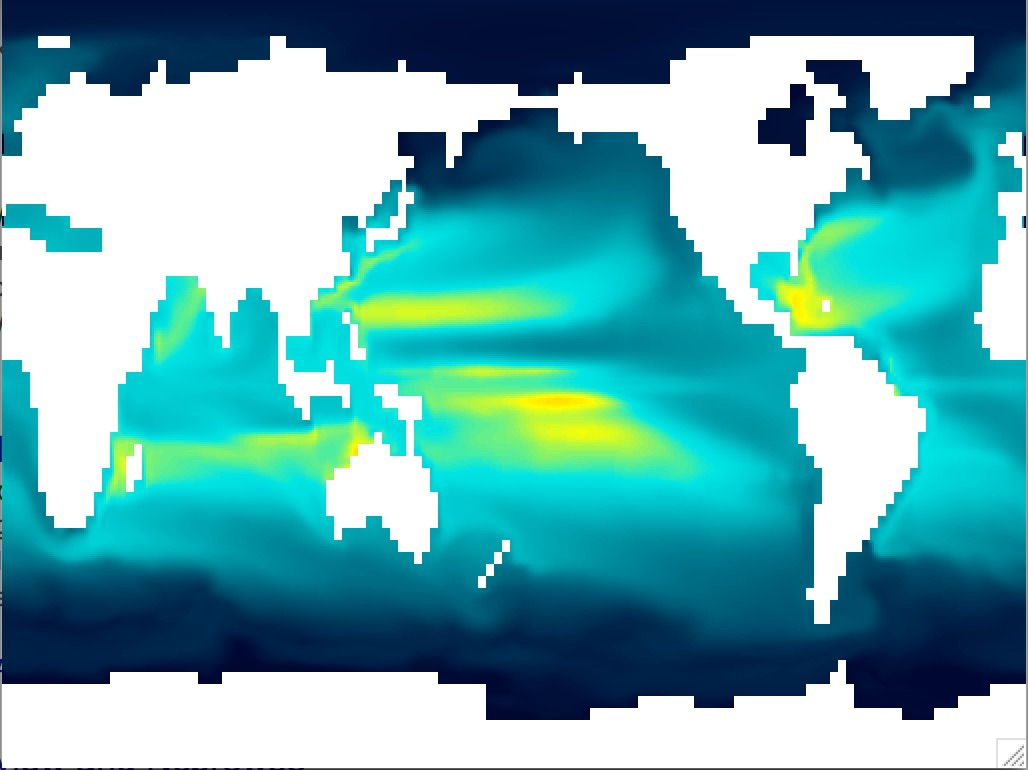
\includegraphics[width=\textwidth]{images/sampling/CanCM4_screenshot.jpg}
        \caption{}
        \label{cmip_example}
    \end{subfigure}
     \caption{Example snapshots of simulation output. (a): Dark matter particles (speed mapped to color: purple is faster) from the final timestep of an Illustris simulation. Note the halos that have formed in dense regions. (Image credit: Illustris Collaboration.) (b): One snapshot of output from SUMO for three lanes (A, B, C) along a stretch of road. At bottom, we see the average speed and its uncertainty, measured at four detector locations (one of the detectors is inactive in lane A) in one time window; in the middle, a snapshot of all the cars along this stretch of road for a single time in the window; at top, a zoomed-in view of the cars very near one detector at this time. In all sections, speed is mapped to the blue scale at left (darker is faster). (c): CanCM4, which is one of the CMIP5 models. Here, the ocean cells at a single depth level, with temperature mapped to color (yellow is warmer; blue is colder), are shown in the netCDF viewer.}
     \label{data_examples}
\end{figure*}

% emphasize the ways in which these simulations have orthogonal properties to one another:

% - different sources of discretization
% - 

% --> claim "transferability to people with the same needs" of the tool (rather than "generality") (do this a bit later in the paper)

\subsubsection{Dark Matter Simulations}
\label{dark_matter}
Our first source is Illustris~\cite{illustris_original},~\cite{illustris_release}, a suite of cosmological simulations. We downloaded the dark matter data from a single snapshot, the final timestep ($z=0$) of a dark-matter-only simulation run, Illustris-3-Dark. In N-body simulations such as these, dark matter mass distributions are represented by discrete particles. This representation approximates the continuous distribution of dark matter in the universe, creating uncertainty known as ``particle shot noise.'' Shot noise inserts uncertainty into all analyses of these simulations.

% also mention the size of the dataset we used, and the size of the biggest Illustris simulation, as well as the size of other n-body DM sims out there

Dark matter halos, which are gravitationally bound groups of dark matter particles that coalesce over time, are interesting partly because they are the environments in which galaxies form.  Algorithms that identify catalogs of halos from time-variant dark matter simulation data are called ``halo finders.'' A wide range of halo finders exists; assessing the quality of their performance is difficult, because there is no clear definition of ``halo,'' and because halos can have complex structures~\cite{behroozi}. However, the results from a halo finder determine the accuracy and usefulness of properties derived from halo catalogs. 

The ``halo mass function'' (HMF), one of these derived measurements, is a histogram of the mass distribution of dark matter halos within a simulation. Particle shot noise uncertainty, which means that the assignment of particles to particular halos is uncertain, and therefore halo masses are also uncertain, leads to uncertainty in the HMF.  Small differences in halo finder results may result in significant differences to the resulting HMFs and to ``merger trees,'' which are plots of how dark matter halos merge together over time~\cite{avila2014sussing}. (For more information on dark matter, halos, and merger trees, see~\cite{lacey1992}.)

As new surveys from telescopes measure cosmological properties to ever-greater precision, the need for accurate measurements from cosmological simulations, and understanding of their bias and uncertainty, becomes even more urgent. For comparison with sky surveys, HMFs measured from simulations need to be accurate to within 1-5 percent~\cite{behroozi},~\cite{tinker}. In order to use the HMF to observationally probe dark matter, cosmologists must continue identifying the sources of, and reducing, uncertainties in theoretical HMF measurements~\cite{murray2013}.
          
\subsubsection{Traffic Simulations}
\label{traffic_sims}
%what are traffic simulations?
% what's the source of uncertainty?
% what are we measuring and what's the significance of it?
% what are some use cases?

Our second data source is SUMO~\cite{SUMO2012}, an open source, microscopic traffic simulation. In this context, ``microscopic'' means that the behavior of each individual vehicle is simulated. SUMO simulates the placement of data-gathering detectors along roadways. Quantities available in our selected dataset include locations of detectors, time and speed of each vehicle when it passes each detector, vehicle length, and lane. Traffic model analysts use derived traffic variables, such as flow rate and vehicle density, to find \textit{spatiotemporal traffic patterns}~\cite{kerner2014introduction}. For example, using traffic models, analysts can quantify a distinction between free flow and congested traffic, then try to identify the causes of jams and congestion.

Traffic models are crucial to transportation planning in a range of situations. For example, traffic models are often used to plan for evacuations~\cite{Pel2012}. Predicted quantities can include number of vehicles involved in an evacuation, their starting points and destinations, and the traffic flow that will result from these conditions. In emergency situations, it is vital to understand the confidence in a given prediction, so that officials can make decisions based on the most likely scenarios.
Quantifying the uncertainties in traffic simulations, however, which come from inputs and from the models themselves, is challenging~\cite{traffic_volume}. One of these uncertainty sources is discretization of differential equations that describe traffic movement. To understand the likelihood of different traffic forecasts, one must understand the influence of uncertainty.
          
\subsubsection{Climate Models}
\label{climate_models}

Our third source is an ensemble of climate models from Phase 5 of the Coupled Model Intercomparison Project (CMIP5)~\cite{taylor2012overview}. Climate models are highly complex, including hundreds of tunable parameters determining the behavior of interdependent physical processes \cite{debusschere}, \cite{randall}. We select an ensemble of nine models: CanCM4, CanESM2, CCSM4, CNRM-CM5, IPSL-CM5A-LR, MIROC4h, MIROC-ESM-CHEM, MRI-CGCM3, NorESM1-ME~\cite{taylor2012overview}. Models are run according to scenarios, called ``Representative Concentration Pathways'' (RCPs), which are possible trajectories for future greenhouse gas emissions. All models in our ensemble represent RCP4.5, which is a scenario of future low-emissions climate policy~\cite{van2011representative}. These RCPs provide a manageable, intuitive set of projected outcomes to analysts and policymakers~\cite{mcsweeney}.

% talk about size of models (and that ours is smaller because we're just using ~1 variable), and potentially larger sizes of other ensembles
The choice of models making up an ensemble is a source of uncertainty.  Most often, climate scientists measure quantities and patterns by averaging over an ensemble of models (``multi-model mean'')~\cite{vavrus}. Uncertainty is defined by the spread of models around this mean \cite{deser}, \cite{georgakakos}. Information about the spread in the models, such as their standard deviation, can help quantify this uncertainty. But the choice of models to include in an ensemble also contributes to uncertainty \cite{knutti}, \cite{vavrus}. For example, results may significantly change with the inclusion of one model in place of another. If a particular model is in disagreement with the consensus of most other models, it is unclear whether to include or exclude this model: its outlier status does not necessarily mean it is wrong, and it may well be within the range of plausible outcomes \cite{mcsweeney}. There may be scientific reasons for excluding a particular model from the ensemble--if it does not realistically represent a key, known climate process--but that analysis is outside the scope of our study; our results may be applied to any group of models with any selection criteria. 

%Several approaches to quantifying this uncertainty due to model choice are outlined in \cite{vavrus}. The authors choose to strike a balance between simple and complex methods using bootstrapping (see Section~\ref{bootstrapping}). They demonstrate that the mean and standard deviation of a bootstrapped, resampled climate model ensemble provide precise information about the confidence level of a prediction. Bootstrapping the ensemble allows for far more nuanced uncertainty analysis than does simply considering the range of values in the models themselves~\cite{potter:2009}

We choose ocean heat content (OHC) for analysis because of its conceptual importance. Ocean heat content is a key indicator of climate change effects \cite{cheng}. It is also mathematically simple: calculating OHC requires integrating heat capacity over every ocean grid cell volume in a model. Therefore, we select our models from among those CMIP5 models with ocean cell volumes and ocean heat capacity data. Models have different spatial resolutions, adding another source of discretization uncertainty. It is important to assess and constrain uncertainty in OHC, as it is closely related to Earth's heat balance, which is crucial to the conclusions of climate change studies ~\cite{cheng},~\cite{gregory}. 

\subsection{Bootstrapping and Simulation Uncertainty}
\label{bootstrapping}
Bootstrapping is the process of randomly sampling a dataset with replacement. One randomly chooses elements of a dataset, allowing elements to be chosen multiple times. Some items, then, will be included more than once, and some will be excluded. Repeating this many times creates an ensemble of datasets useful for estimating variance of the source dataset~\cite{Steck}. Thus, bootstrapping provides a simple, generalizable, powerful way to quantify uncertainty. 

For example, bootstrapping techniques have been used  in~\cite{rau} to estimate the effect of particle noise in N-body simulations. Researchers use N-body simulations to study gravitational lensing, a phenomenon in which light is bent around a massive object in space. The authors of~\cite{rau} create a dataset with 100 bootstrapped resamplings, each containing the same number of particles as the original dataset; this allows them to test the effect of particle noise on the lensing in the simulation.

Bootstrapping has also been used to estimate uncertainty in measurements of climate models. As discussed in Section~\ref{climate_models}, the multi-model mean used to assess climate ensembles introduces uncertainty. The authors of~\cite{vavrus} use bootstrapping, resampling from an ensemble of 13  models, to assess the uncertainty of temperature and precipitation measurements. Similarly, bootstrapping has been used to estimate uncertainty in traffic forecasting models~\cite{RePEc:eee:transa:v:39:y:2005:i:6:p:531-547},~\cite{Brundell2000}.

Differentiating among uncertainties in climate simulation data based on their sources is quite difficult. Bayesian models may be used to determine the contribution of each source of uncertainty~\cite{northrop}, but in general, the complexity of uncertainties in interacting processes can occlude one another. Bootstrapping over the choice of models provides a conceptually elegant way to assess the effect of the model choice on uncertainty. This is true, too, for particle noise; bootstrapping will allow us to extract and quantify the uncertainty resulting from particle noise. 

A bootstrapping and sampling procedure has the advantage of being strongly generalizable. These techniques can be performed without any prior modeling of the data. Additionally, sampling can be improved on-the-fly; if a certain number of samples does not give satisfactory results, one can increase the number of samples as desired without having to start over~\cite{Cormode:2012:SMD:2344400.2344401}.

\section{Methods}
We outline the steps taken to measure and model discreteness uncertainty for each dataset, aiming to develop a generalizable procedure. 

\subsection{Sampling}
First, we extract samples of size $f$ from each dataset, for a range of values of $f \ll 1$. Table~\ref{speedup_table} shows the sample sizes used in our case studies; these samples were chosen to be small enough for significant speedup, while large enough to capture sufficient information (see Section~\ref{results}). For the particle data, we randomly select $f * n_p$ particles, where $n_p$ is the total number of particles in the simulation. From each climate model, we extract $f * n_c$ cells, where $n_c$ is the total number of ocean cells in a model, and from the traffic model, we extract $f * n_o$ observations, where $n_o$ is the number of traffic detections. While the mass per particle is constant in Illustris-Dark, the CMIP models have different numbers of ocean cells, and total ocean volumes vary. Therefore, a dark matter sample of size $f$ includes a total particle mass of $f$ times the total particle mass, while an ocean model sample of size $f$ does not necessarily have a volume equal to $f$ times the total ocean volume.

Next, we must identify the independent variables for each dataset: 
we will want to know the uncertainty at points in this parameter space.
For the halo mass function, these values are mass bins; for ocean heat content change, these are timesteps (monthly); and for average traffic speed, these are positions of detectors.

%We determine a number of domain bins, sample points, etc., for each dataset, or assign an algorithm to automate this decision. This is straightforward for the climate model data, which in our case is divided into monthly timesteps. In our first modeling attempt with the dark matter data, we set uniformly spaced mass bins. In order to ``smooth'' our input data for improved modeling---so as not to overfit the data---we set the number of bins to half as many as were automatically chosen by the yt halo finding algorithm \cite{yt}. This provided good spacing for larger mass bins, with smoothly varying values between mass bins at various sampling sizes. For the smaller mass bins, however, the measurements---i.e., the number of halos larger than these masses---had high values that varied greatly between adjacent mass bins and were wildly inconsistent depending on the sample size. Thus, we use adaptive mass binning (TO DO.)

\subsection{Uncertainty Measurement}
Next, we estimate the variance in the relevant measurement, for each sample, using the following procedure:

\begin{enumerate}
\item Use bootstrapping to resample the sample once.
\item Perform the relevant measurement (HMF; OHC; average speed) on this resampled data.
\item At each timestep/mass bin/position, measure the variance of all measurements we have taken so far.
\item Repeat (1-3) until the variance converges at most timesteps, mass bins, or positions.
\end{enumerate}

%can include table of number of resamples & epsilon values for each application + fraction.

Because the total mass in the Illustris samples varies with fraction size, we use relative mass values, first measuring the range of halo masses for each halo catalog, then dividing this range into equally-spaced steps. Through trial and error, we find that sampling masses regularly along a logarithmic scale provides smoothly varying, and consistently-shaped, halo mass functions.

Step 2 is highly domain-specific. To obtain halo catalogs for each dark matter subset, we modify the yt halo-finding library~\cite{yt} to find halo measurements at our specified mass bins. This yields, for each bootstrapping iteration, a value for halo number density at each mass bin, which is the halo mass function (HMF). 

For the climate data, we measure ocean heat content (OHC) for each bootstrapping iteration by integrating over the heat capacity for each ocean cell, then taking the multi-model mean, for each timestep. To account for the varying ocean cell volumes, we normalize these values using the ratio of the sampled volume to the total ocean volume in each model. This yields, for each bootstrapping iteration, an OHC value for each timestep. We then calculate the change in OHC with respect to a reference time, which is the format that scientists most often study.

Lastly, for the traffic data, we simply average the speeds measured at each detector in our sample, within time bins. This yields an average speed at each detector for a range of time windows.

For each of these measurements, we check the variance in each timestep or bin by plotting the variance per iteration and measuring the threshold of variance (i.e., the number of iterations N after which the range of values is within some value $\epsilon$). Once we have calculated the OHC or HMF over enough iterations to have reached convergence in most mass bins or timesteps, we store the bin/timestep, variance, minimum, maximum, and median values, and 25th and 75th quartiles. These comprise the five summary statistics of uncertainty often depicted in boxplots~\cite{brodlie2012review}. 

%FIGURE: boxplots (in my interface) of results so far for each application, or just for one if not enough space.

\subsection{Kernel Regression and Extrapolation} 
\label{methods}
%this section most recently edited by yiran:
Next, we aim to learn a model, $\mathcal{M}$, for predicting the uncertainty of each measurement on the full datasets, using the information we have gathered as input:
\begin{equation}
\mathcal{M}(u_f, f, x) = u_{1.0}(x)
\end{equation}
where $u_f(x)$ is the uncertainty at $x$ (i.e., some timestep or mass bin) for fraction $f$. We represent uncertainty using the \textit{five-figure summary} of distributions found in boxplots: minimum, maximum, median, lower quartile, upper quartile. To reduce the dimensionality of the problem, we learn five models, one for each of these quantities. Ideally, we can save a model, once learned, then use other datasets---for example, samples from a similar simulation run---as input. 

	To predict the value of responses, given predictors, and estimate the associations among predictors and responses, one can use regression techniques. Our predictors are the uncertainties of a small data subset, and our responses are the ground truth (the uncertainties of the corresponding full dataset.) Parametric regression fits a functional form to the model inputs and outputs. This would be conceptually elegant for inserting new data into the model inputs and calculating the outputs. However, choosing a functional form to fit would be difficult without intuition for what shape the uncertainties of a dataset should take. Nonparametric modeling has the advantage of more degrees of freedom, sacrificing the elegance of a functional form---which may not be generally applicable to many types of scientific data---for greater predictive power. 

%NOTE: how do we allow substitution of a new dataset into the model?
%%%
One difficulty is that our model requires extrapolation. That is, the inputs for $f$ include values $f \ll 1.0$, but we would like to predict the output at $f = 1.0$, far beyond the range of inputs. In our case, extrapolation is motivated by the fact that the ground truth's uncertainty-related values usually share a similar pattern with those values for smaller fractions (see results in Section~\ref{results}.)

Recent work~\cite{pmlr-v28-wilson13}~\cite{WilsonGCN14} explores the challenge of extrapolation, proposing fast kernel-based regression approaches for performing extrapolation. However, the distance between training and testing inputs in our case is especially long; additionally, we expect that the uncertainty (both its magnitude and its relative values) can be strongly dependent on the sample fraction. This burdens even the best methods for predictions based on spectral mixture kernels. 

%\subsubsection{Data Preprocessing}

%First, we determine how to scale the uncertainty-related values (minimum, maximum, median, lower quartile, upper quartile) and the independent variables. 
% For example, a linear regression was performed for each fraction after the HMF data was logarithmized. 
%(NOTE: we didn't have to do this step for the other applications.)
%In order to make a clear distinction between the effects of two input variables, the linear regression parameters were recorded and then used for normalization. Mathematically, the linear regression equation for fraction $f_i$ is:

%\begin{center}
%$log(u_{f_i}) = A_ix + b_i, i = 0, 1, 2, \dots, n,$  
%\end{center}

%where $x$ is the mass bin index, and $n$ is the number of input fractions. In order to eliminate the influence of fractions on the other input feature, the mass bin indices, the data was then normalized to be of the same linear equation:

%\begin{center}
%$u'_{f_i} = (log(u_{f_i}) - b_i) \times (A_0/A_i) + b_0$
%\end{center}

To improve the extrapolation performance, we tested different ways of scaling the model parameters, ultimately making choices based on trial and error. We aim to bring the features near enough to accommodate kernel learning in the following step, but not to distort the data so much that floating point arithmetic becomes a factor. Our interface is designed to assist users to make these scaling choices (see Section~\ref{vis}) based on simple equations. For each case study, we scaled the sizes with equations of the form $\mathrm{scale}_{\mathrm{f}}(f) = \mathrm{log}(f^{1/c})$. Depending on the domain, the independent variable (such as mass) may also be scaled in order to serve as a consistent reference for different sample sizes.

To train the model with sampled data, we use pairs of sample uncertainty as the ``input'' and ``output'':

\begin{equation}
%\begin{align}
%\begin{split}
\mathcal{M}(\mathrm{v}_f, \mathrm{scale}_{\mathrm{frac}}(\mathrm{input\textunderscore frac}), \mathrm{scale}_x(x)) = \mathrm{v}_{\mathrm{output\textunderscore frac}}(x)
%\end{split}
%\end{align}
\end{equation}

for each value, $v$, representing uncertainty being predicted. In this study, the values used are the minimum, maximum, median, lower quartile, and upper quartile. To make predictions, we will use the model in Equation 2 with the output fraction set to 1.0 and the input being the array of training samples. 

%A scheme was designed to assist the user in defining the scaling method. Choices of exponent $c$ are made by the user, and then a scaling process and a linear regression was performed based on the chosen exponent. The efficiency of the scaling process is then illustrated by the RMSE of the regression.

\subsubsection{Prediction}
We first arrange input fractions and independent variable indices of the training samples as data points on a grid. We adopt gaussian process methods for extrapolation, closely following the method in~\cite{pmlr-v28-wilson13}. A kernel (covariance function) is selected to represent the distribution of a set of functions, and then a posterior is generated according to the training data. Based on the posterior distribution, predictions are made for the ground truth data.

% don't know whether the formulae are needed here
The spectral mixture kernel, $k_{SM}$, we use is:
\begin{center}
$k_{SM}(x, x'|\theta) = $$\sum_{q=1}^{Q}$$w_q^2\frac{|\Sigma_q|^\frac{1}{2}}{(2\pi)^\frac{D}{2}}\exp(-\frac{1}{2}||\Sigma_q^\frac{1}{2}(x - x')||^2)$\\ 
$\times\cos(x - x', 2\pi\mu_q),$
\end{center}

where $\theta$ represents all of the kernel hyperparameters, and one SM kernel is defined and initialized for each input dimension. To learn the hyperparameters, we maximize the log marginal likelihood:
%The hyperparameters can be learned by maximizing the log marginal likelihood:
\begin{center}
$\log(p(y|\theta, X))\propto -[y^\mathrm{T}(K_\theta + \sigma^2I)^{-1}y + \log|K_\theta + \sigma^2I|].$
\end{center}

%We also don't want very different fractions to be too close to one another. 
%to add: is there a way to know while we're tuning this that our choice is a good one? any information available?

%IMAGE: optimized scalings in the interface, for one example.

%discuss multi-scale properties/difficulty:

%Some of these quantities change with varying subset sizes, such as mass, halo number density, and the magnitude of ocean heat content, while some, such as timesteps, don't. Downsampling the data means that though the variance of a quantity in a subset may be roughly proportional to the variance of that quantity in the full dataset, the absolute values will not be the same. For example, when we downscale, the range of halo masses decreases. For our model, we'd like to convert between these masses to the masses found in the full dataset. This will be true of any property that is directly affected by downsampling, such as number densities. Ideally, this scaling can be hidden within the model, which will learn the relationship between input and output values. However, we may have to explicitly scale values if the models do not address this adequately (TO DO).

We run each model to make five predictions, one for each value in the uncertainty spread (five-figure summary). %(Note: is there a better way to learn a distribution??) 
To apply the trained model to a new dataset, such as another simulation run using different parameters, we save the learned parameters and apply them to the new dataset. See section~\ref{ohc_case_study} for an example result.

\subsection{Visualization}
\label{vis}
%THESIS OF THIS SECTION: visualization is crucial to the applicability of our tool. our method is fast so that it enables real-time prediction, and visualization facilitates exploring this prediction AND it also facilitates tuning to more-precise predictions if desired.

%boxes showing convergence quality: striking the balance between too much information -- can have infinite layers of uncertainty if we look hard enough -- and just hinting at the relevant information.

%make sure to gather sources that specifically pertain to this section.

% list what we want users to be able to do/see in our visualization:
Visualization enables the full usefulness of our approach. Through a flexible interactive interface, users can take advantage of its fast prediction and interactive tuning to efficiently explore their own data. Moreover, much of our method's benefit is qualitative: learned patterns in the uncertainty reveal themselves quickly through visualization. Scientists who work with simulations confirm that this kind of information is highly useful (see Section~\ref{uwp}).

Our visualization should enable users to answer the following questions: What is the predicted uncertainty? How confident can we be in the prediction? What are the patterns in uncertainty, depending on sample size? If we change the input, for which values is uncertainty most affected?

Additionally, it should show users enough information so that they can guide the training of an accurate uncertainty prediction model. Our interface contains panels for selecting input data, scaling and optimizing features for modeling (Figure~\ref{control_panel}), and viewing sampled and predicted results (see Figure~\ref{hmf_case_study}). 

%In the left panel, users choose sample sizes to extract, and specify which to include in the model. In the middle panel, we display the distributions of features to be included, allowing the user to scale these distributions as desired. Finally, the panel on the right shows uncertainty measured from the subsamples, and/or the predicted ``true'' uncertainty, in a boxplot-style representation. We indicate confidence in each prediction with a grayscale box representing convergence of uncertainty values for that bin; darker gray corresponds to higher confidence (i.e., better convergence).

The ``control panels'' (Figure~\ref{control_panel}) facilitate all the steps leading up to an uncertainty prediction. First, the user can load a dataset and specify the sizes of samples they wish to extract. Then, the user can ask to perform a measurement of interest by pressing ``calculate.'' This performs the measurement, such as halo mass function or ocean heat content, repeatedly, keeping track of the variance in the results. The calculation is repeated until satisfactory convergence is reached in a majority of the mass bins or timesteps (the desired convergence threshold can be changed as needed).

Once the calculations are performed, the resulting measurement and its uncertainty is shown in colored boxplots, as in Figure~\ref{hmf_case_study}. These can be viewed individually or stacked, with one color representing each sample size. Beneath the boxplots, a box indicates the quality of the prediction (based on the convergence of the variance measurements), with darker gray  indicating higher confidence. The right side of the control panel now shows the distribution of each relevant variable (see Figure~\ref{control_panel}). At this point, users can choose to scale these features, which become inputs into the prediction model, either by using default log scaling, or by typing in the scaling they prefer. This scaling should bring input features closer together for better regression results (see Section~\ref{methods}). In our case studies, we focus on scaling the ``size'' feature.

%\begin{figure}[h]
%    \centering
%    \includegraphics[width=0.45\textwidth]{placeholder_sample_ohc.png}
%    \caption{Our prototype interface. In the left panel, users choose sample sizes to extract, and specify which to include in the %model. In the middle panel, we display the distributions of features to be included, allowing the user to scale these distributions %as desired. Finally, the panel on the right shows uncertainty measured from the subsamples, and/or the predicted ``true'' uncertainty, in a boxplot-style representation. We indicate confidence in each prediction with a grayscale box representing convergence of uncertainty values for that bin; darker gray corresponds to higher confidence (i.e., better convergence). (See Figure~\ref{hmf_predicted} for another, larger interface image.)}
%     \label{ui}
%\end{figure}

Once the array of samples is chosen and the features are scaled, the user can choose ``update prediction'' to train the model and view the predicted uncertainty (for example, as in Figure~\ref{hmf_predicted}).

\begin{figure}[h]
    \centering
   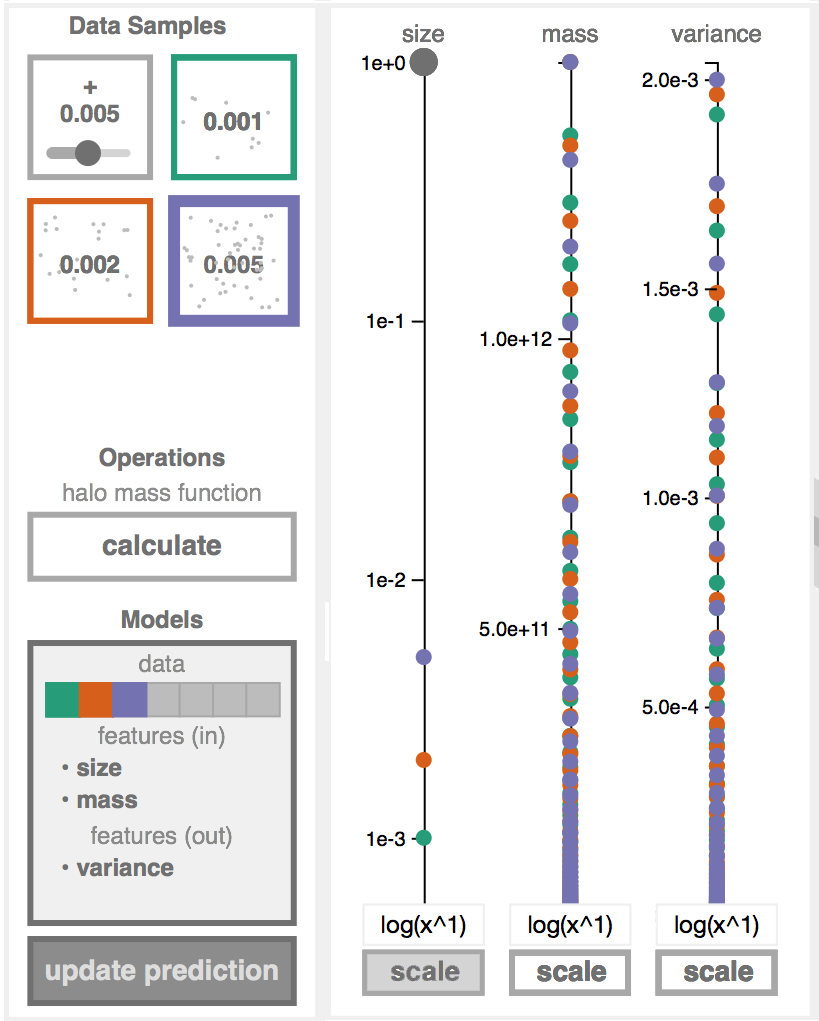
\includegraphics[width=.3\textwidth]{images/sampling/control_panel.png}
    \caption{The ``control panels'' for our interface. On the left, users can choose the sizes of data samples to extract; the ``models'' show which samples and which features are included as input and output to the model to be trained. On the right, the user has scaled the ``size'', or input fraction, parameter.}
    \label{control_panel}
\end{figure}

The default appearance is important, because users might be dissuaded if they have to perform complex interactions before seeing a meaningful result. The fine tuning of our regression model depends on several choices, but the basic implementation of our approach (see Section~\ref{methods}) can provide an estimate of the uncertainty without supervision. We show this estimate by default, allowing the user to then modify feature scalings to optimize the prediction.

% talk about UI components

% talk about problem of comparison

% talk about problem of multiple scales

% TO DO: talk about how to highlight changes

\section{Results and Applications}
We evaluate our method and visualization tool through interviews with scientists working on simulations and three case studies. First, we establish the current work practices of scientists working with simulations, including understanding any visualization tools they use and what needs are not met by those tools. Then, we aim to understand which capabilities of our tool would be useful to them, and the scenarios in which they might use it. Finally, we demonstrate the use of our method and tool on three representative datasets (described in Section~\ref{data}).
%emphasize transferability to people with similar analysis needs

%What's the advantage, if any, of looking at the uncertainty for the measurements on the subsets?


%NOTE: we could discover that the results aren't good in ___ domain but are good in ___ domain (hopefully), and that the application makes sense in ___ domains but not ___ domains, and those may not be the same categories. but if we present those results systematically, it will be convincing.

\subsection{Understanding Work Practices}
\label{uwp}
% cite sources to justify how we did evaluation:
% - "a systematic review on the practice of evaluating visualization"

% identify state-of-the-art for quantifying this type of uncertainty in each field, and qualitatively compare

% to be strong, we need to assess both visualization and data analysis process, with emphasis on the latter

\label{hmf_case_study}
\begin{figure*}[h]
      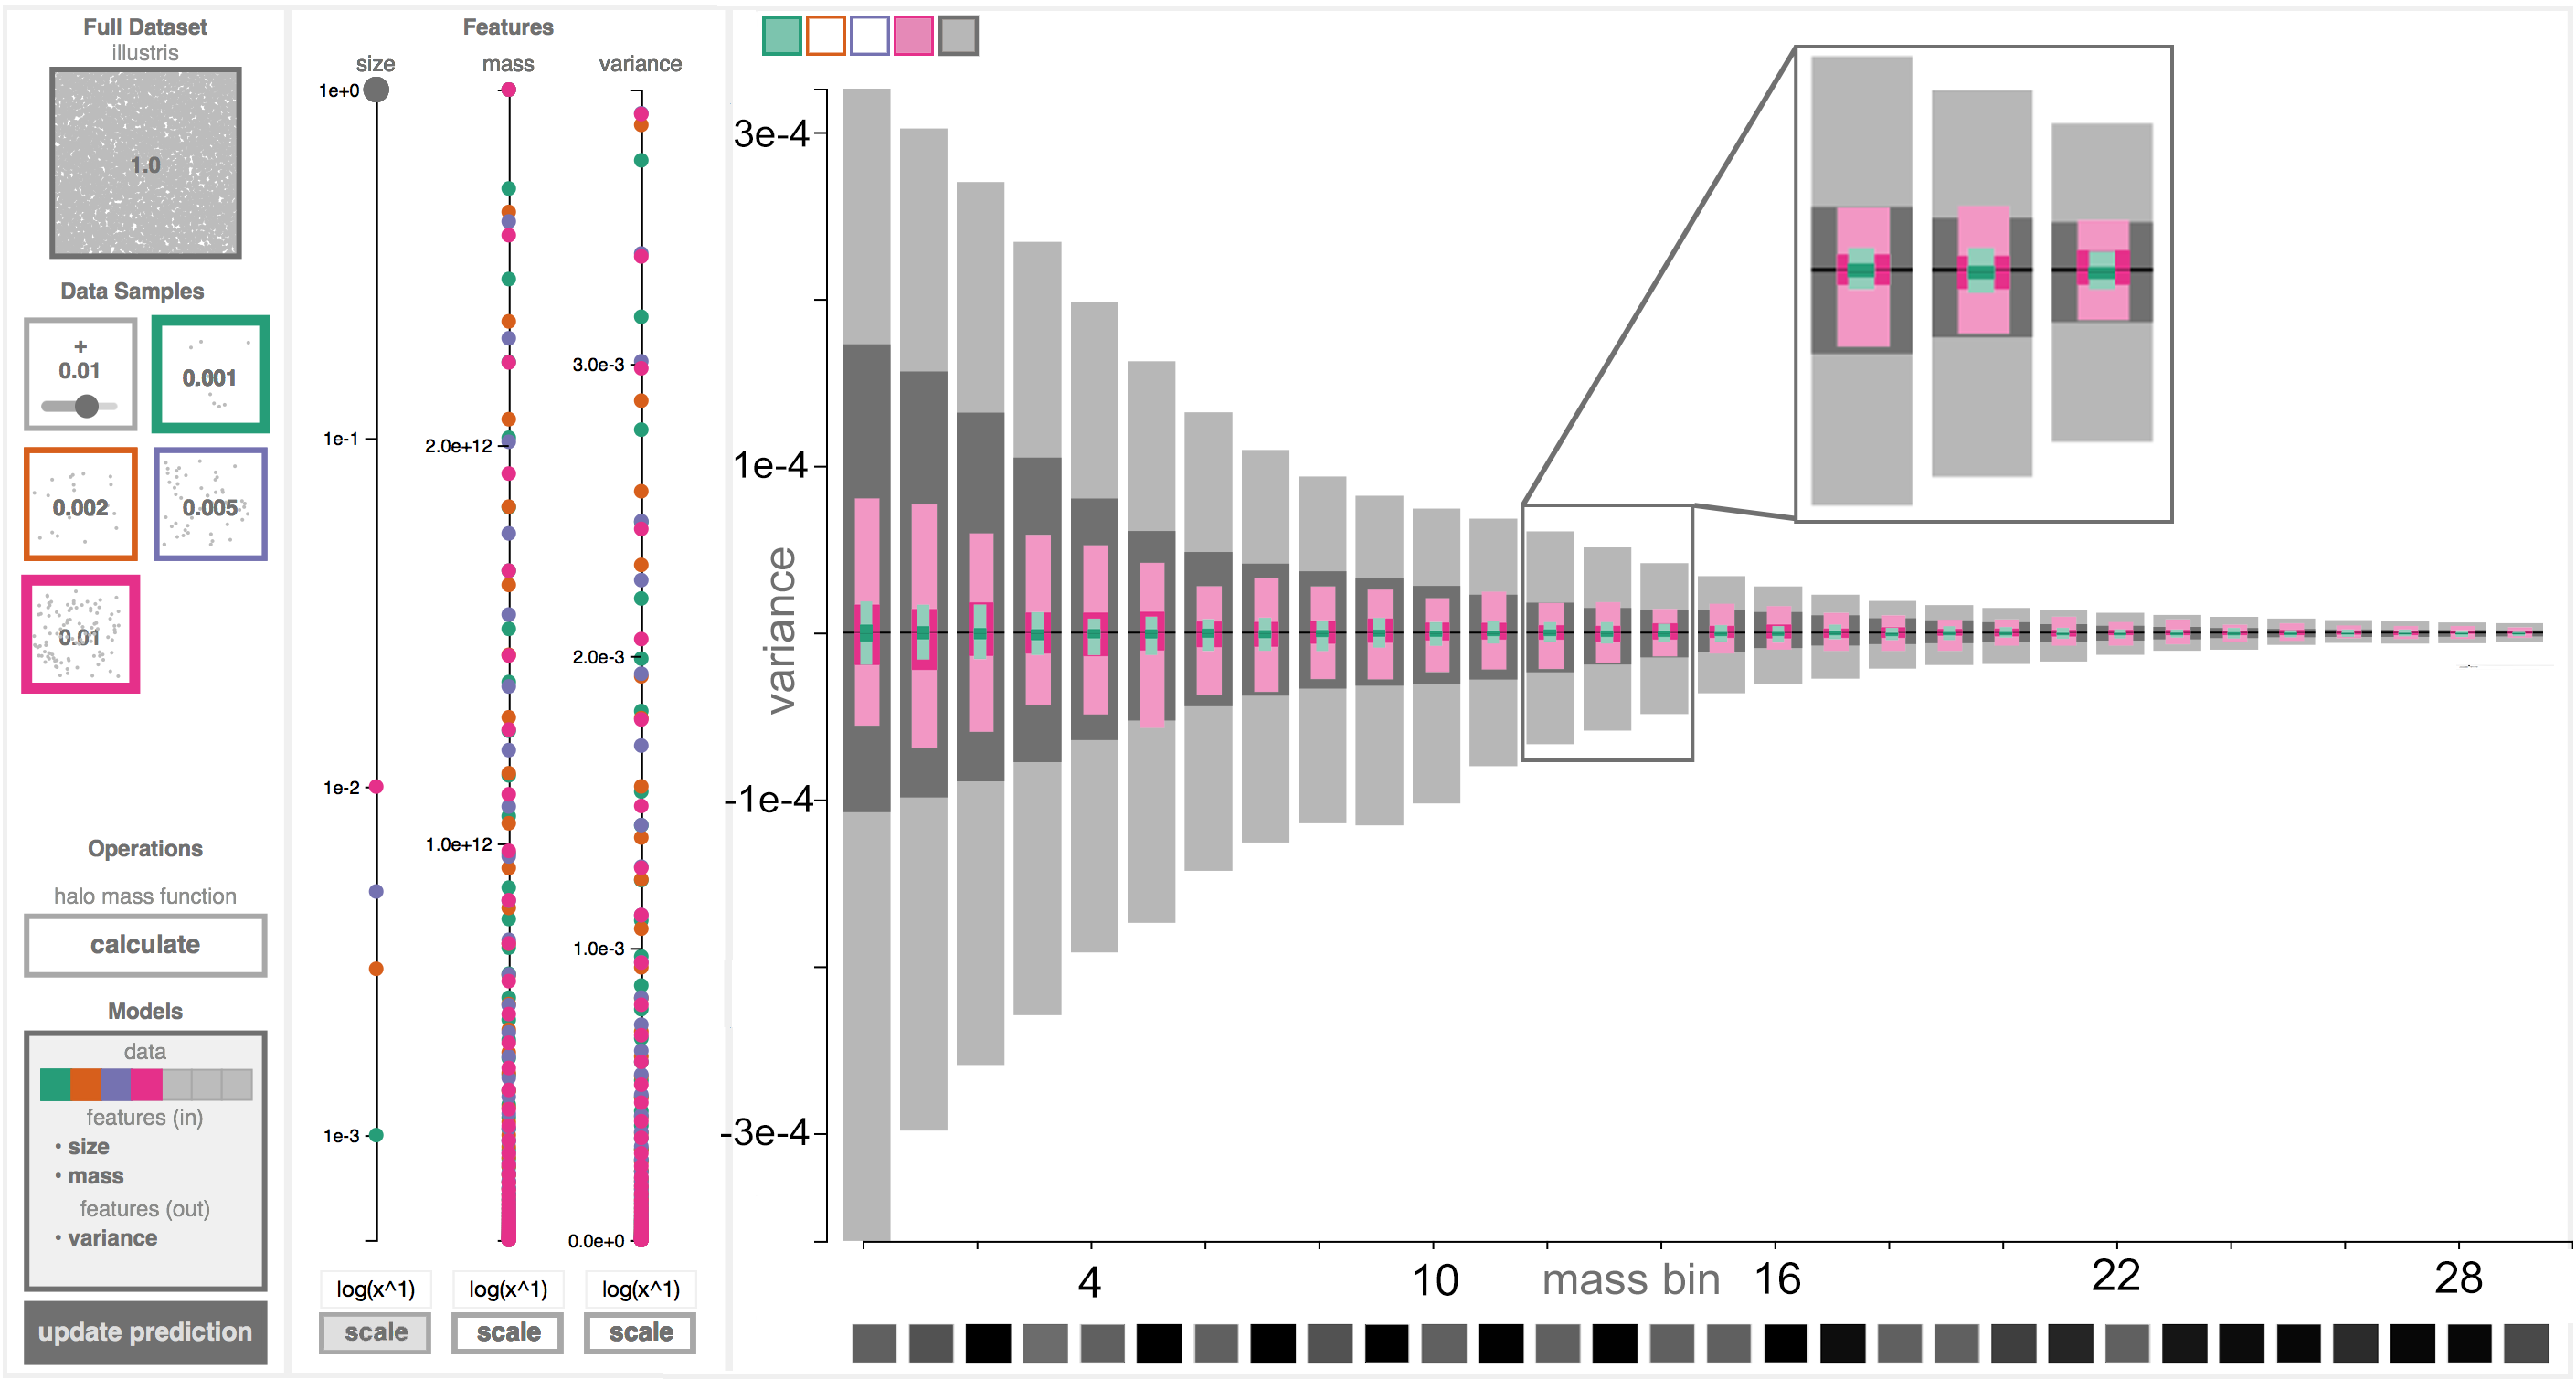
\includegraphics[width=\textwidth]{images/sampling/hmf_prediction_case_study.png}
     \caption{Prediction, and sampled uncertainties, for the dark matter halo case study, shown in our full interface. At left, we see the set of samples the user has chosen. The user has highlighted two samples to show in the uncertainty view. In the middle panel, we see that the user has scaled the ``size'' values as input into the prediction model. At right, we see the measured uncertainties for the samples (pink, green), and the predicted uncertainties (gray), shown in stacked boxplots. Because the halo mass function spans several orders of magnitude, it is difficult to show in one view; instead, we are showing the boxplots centered around their medians for each mass bin. The quality indicator boxes on the bottom of the right panel show that most predictions have a very high confidence. (Axis labels are enlarged for display purposes.)}
     \label{hmf_predicted}
\end{figure*}

To assess the potential usefulness of our approach and visualization tool, we consulted with domain experts who work with climate models and dark matter simulations. Specifically, we spoke with: one Cosmology researcher at a university, in person, who primarily works on N-body dark matter simulations; one Cosmology researcher at a university, in person, who works with observational data but in tandem with other researchers using simulations; one Atmospheric Science researcher at a national laboratory, in person, who primarily works with ocean dynamics in climate models; one Atmospheric Science researcher at a university, over e-mail, who primarily works with ensembles of climate models.

We held these conversations with the goal of understanding common work practices in fields for which simulations play a crucial role. According to a recent survey of evaluation practices in visualization~\cite{6634108}, process-based evaluation such as understanding work practices is crucial yet under-utilized. Through this analysis, we can draw a clear link between our method and tool and the real-world scientific problems it may be applicable to solving.

\subsubsection{Current Tools}
None of the interviewees currently uses visualization tools beyond those offered in R or Python libraries. Several expressed that visualization software is never used in their peer groups, or that visualization is an afterthought, especially for analysis. The reason most cited for this was time, but also lack of a flexible enough tool; one had tried to use ParaView but felt he was unable to use it to show derived properties of his data, and especially not to show uncertainty.

They are all familiar with boxplots or contour plots for conveying uncertainty, and some produce these plots themselves. One person mentioned that he creates his own ``animations'' from series of Python-generated plots. In general, they perform their own statistical analysis using generic packages in R or Python. One atmospheric scientist expressed that the current level of formality in his analysis varies widely, depending on the case; sometimes, statisticians might help with a problem, but they are unlikely to have any expertise in climate modeling. One researcher mentioned using machine learning to explore the parameter space of simulation inputs (see below).

\label{traffic_case_study}
\begin{figure*}[h]
    \centering
    \begin{subfigure}{0.32\textwidth}
        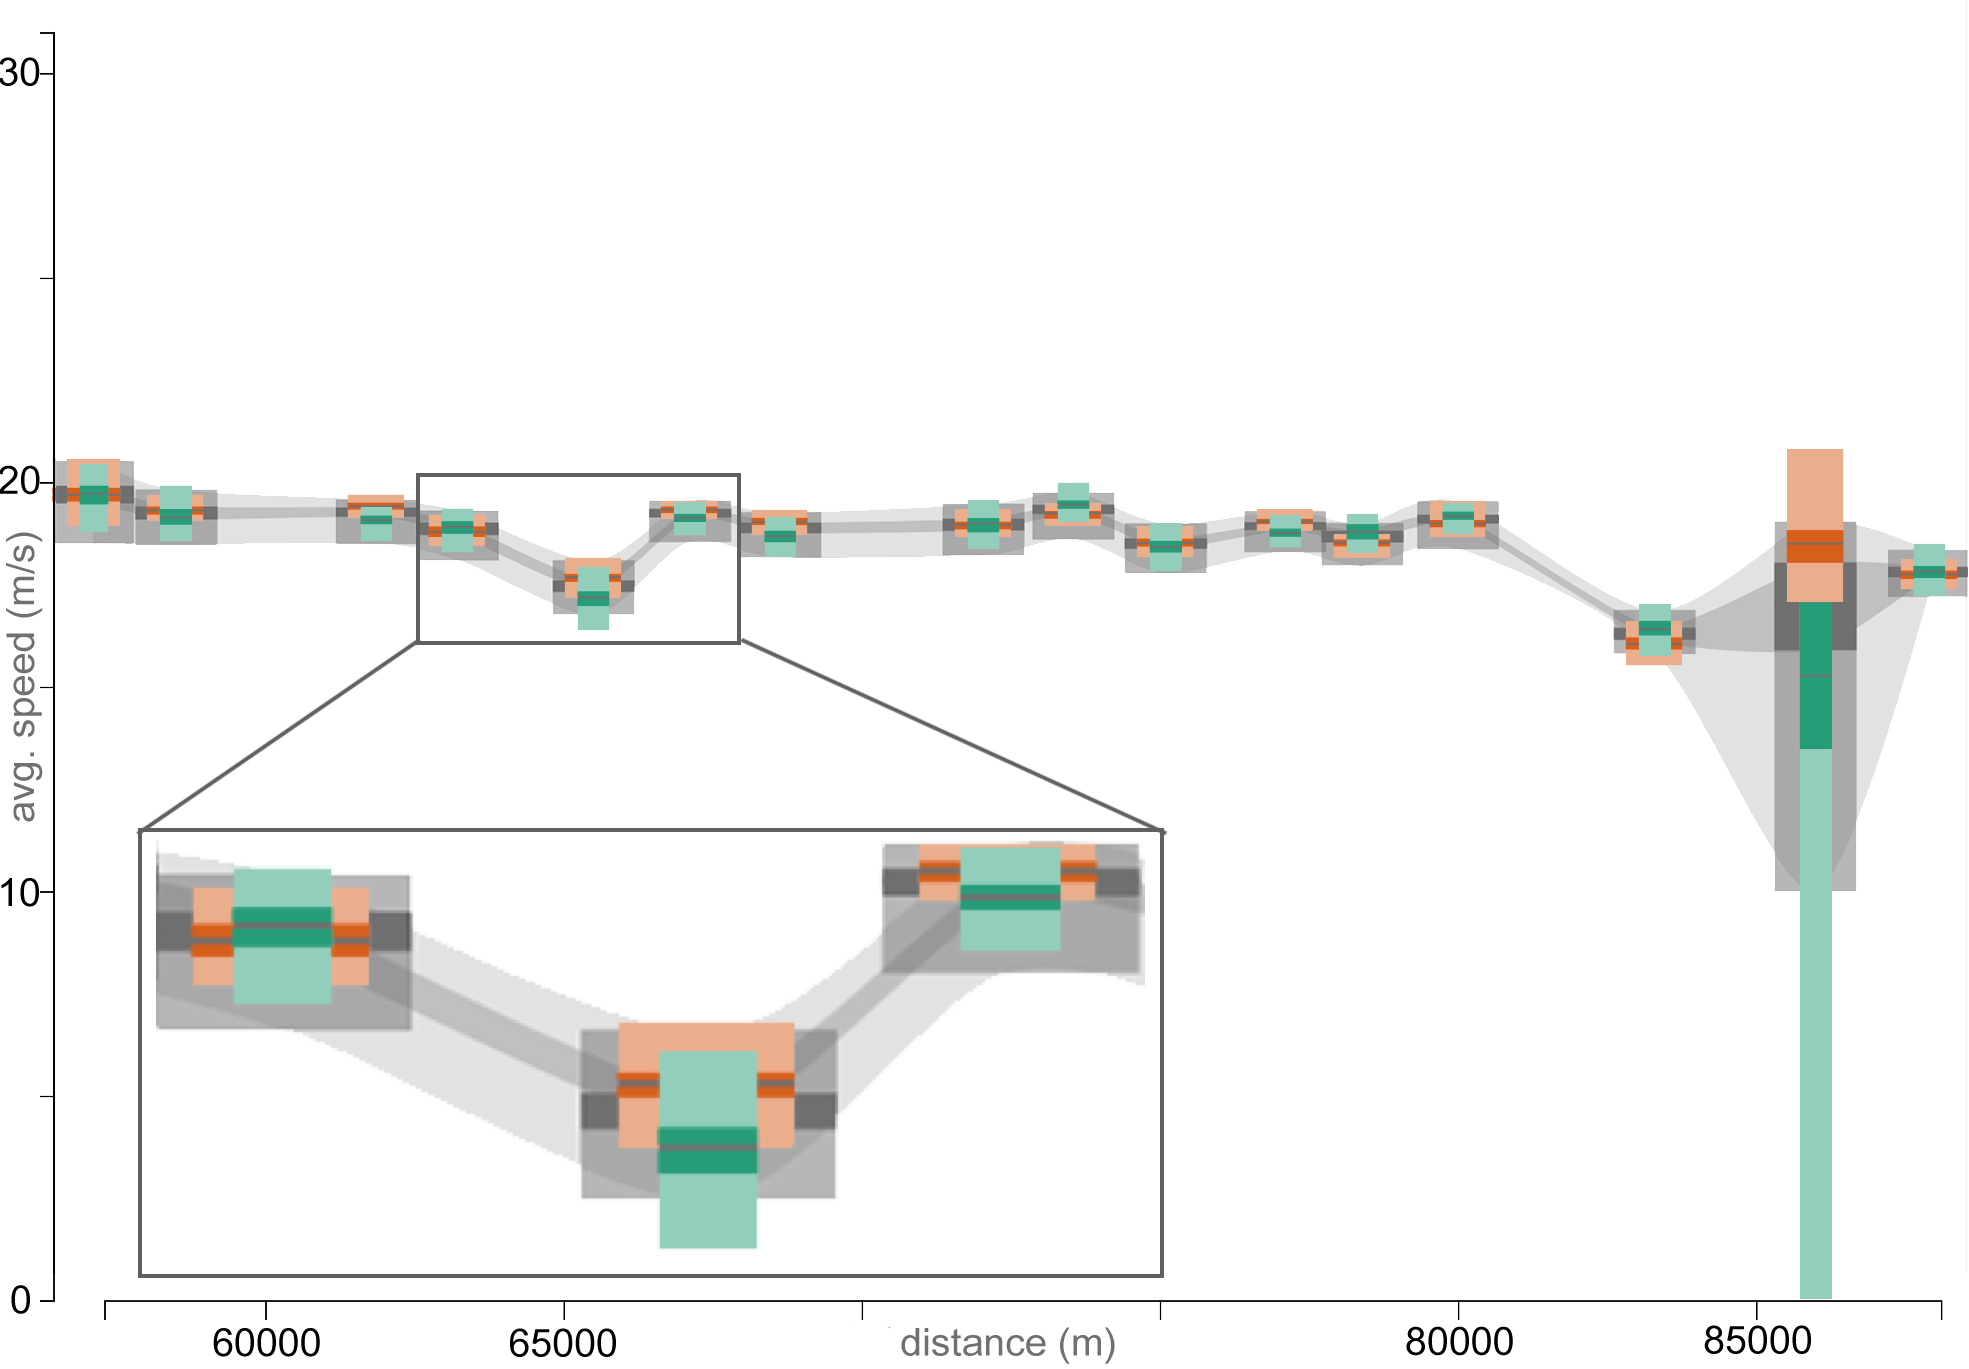
\includegraphics[width=\textwidth]{images/sampling/timestep_a_samples_predicted.png}
        \caption{Time window 1.}
        \label{fig:a}
    \end{subfigure}
    \begin{subfigure}{0.32\textwidth}
        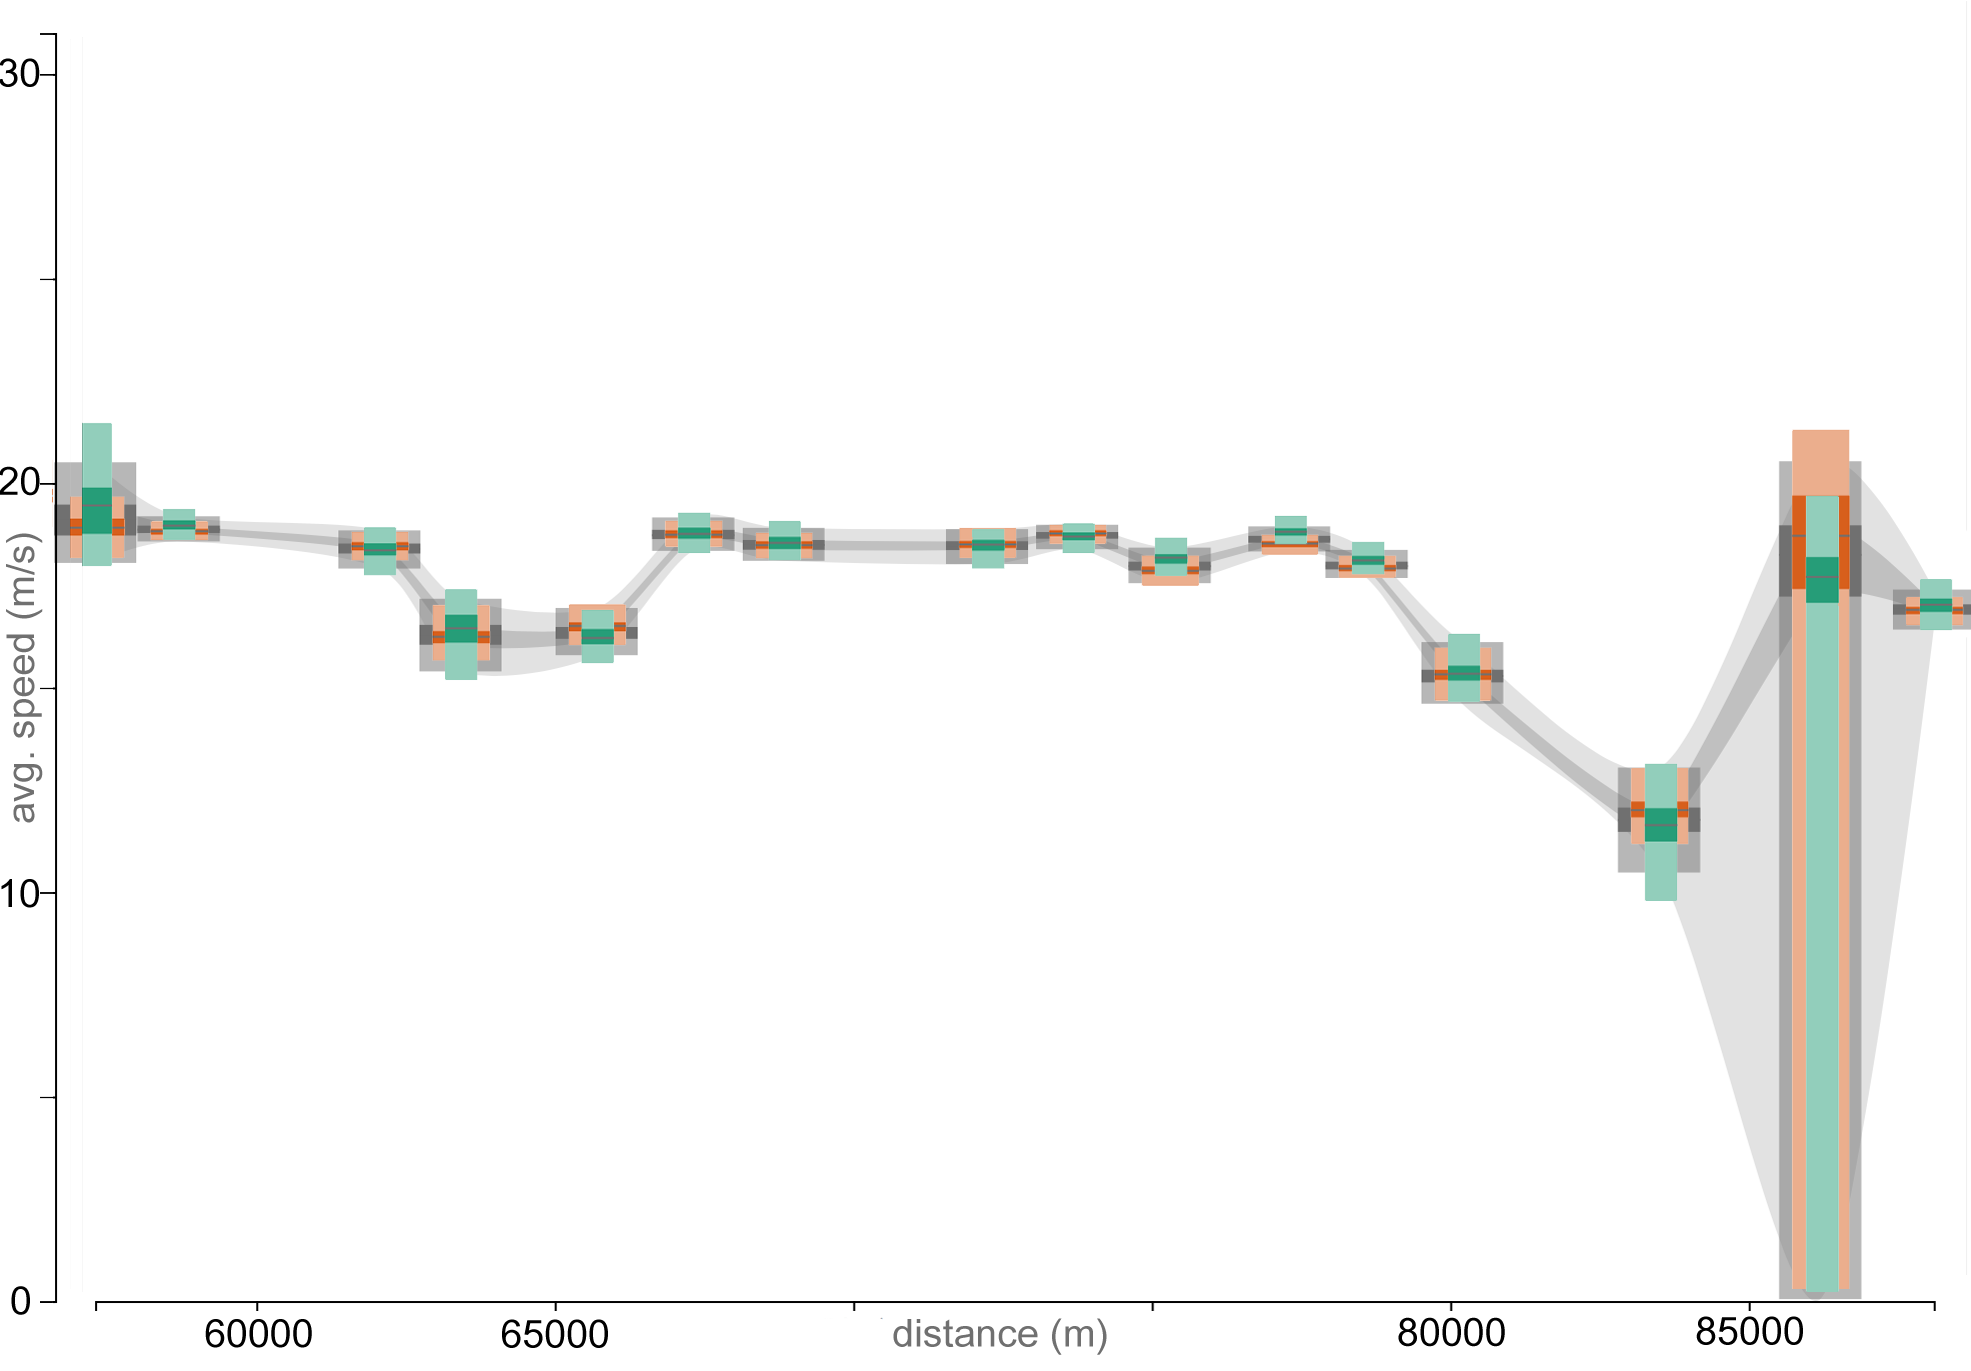
\includegraphics[width=\textwidth]{images/sampling/timestep_b_samples_predicted.png}
        \caption{Time window 2.}
        \label{fig:b}
    \end{subfigure}
    \begin{subfigure}{0.32\textwidth}
        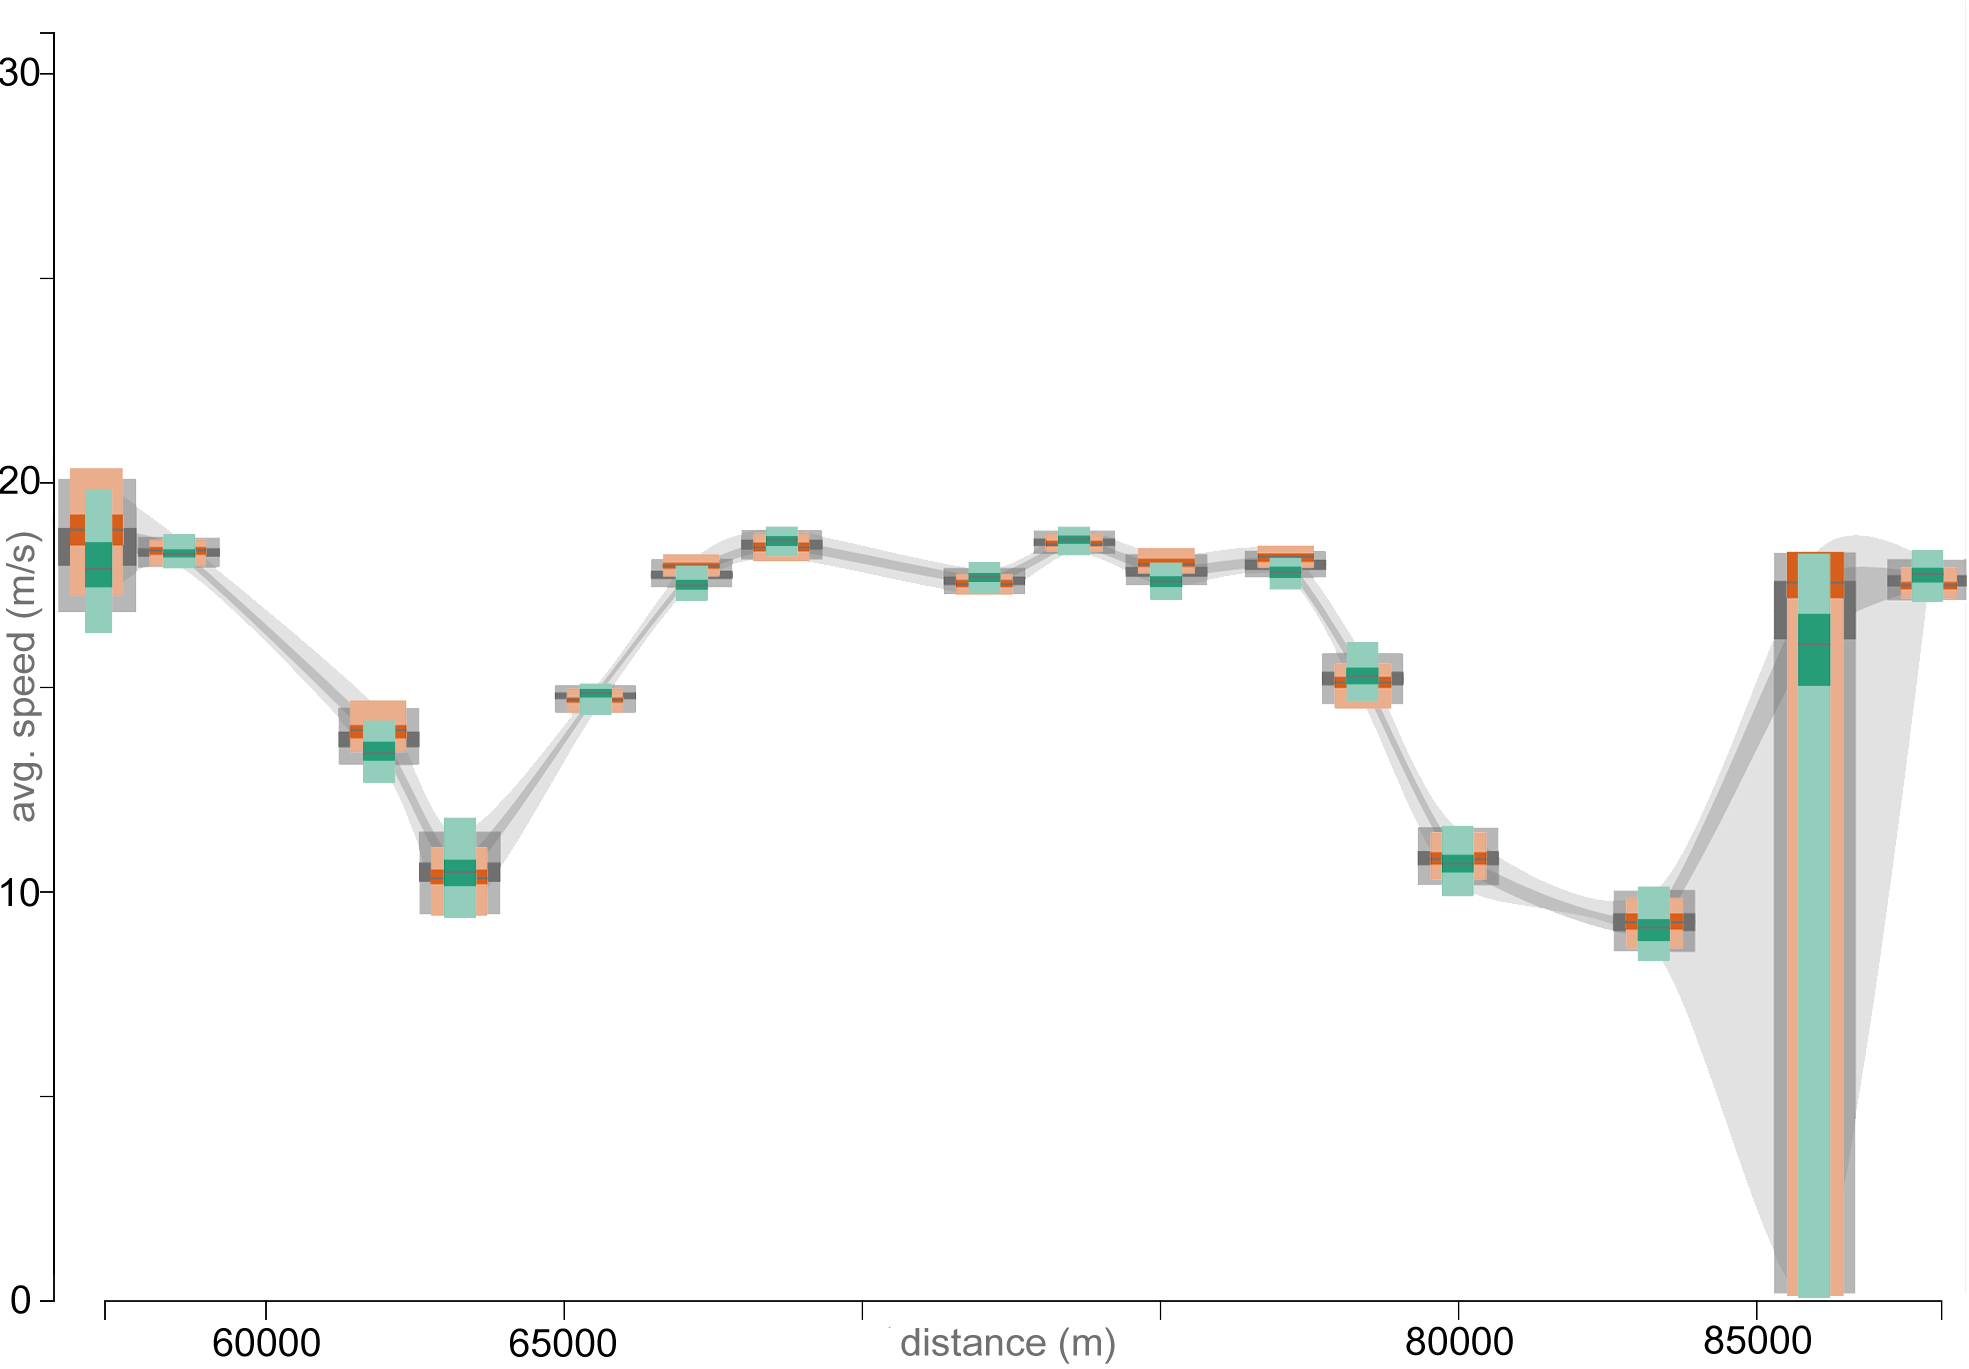
\includegraphics[width=\textwidth]{images/sampling/timestep_c_samples_predicted.png}
        \caption{Time window 3.}
        \label{fig:c}
    \end{subfigure}
     \caption{Average speed and uncertainty for samples with sizes 0.05 (green) and 0.1 (orange), and the predicted uncertainty (gray, connected by an interpolated curve), for three consecutive time intervals. The interpolated curve of predicted values helps discern the path of a time series, especially when the samples are unevenly spaced, as in this example. The inset box in (a) shows the overlaid boxplots in detail. Here, the green box, representing sample size = 0.05, represents the median (middle gray line), upper/lower quartiles (darker green), and min/max (lighter green). Similarly, orange ($f=0.1$) and gray (prediction, $f=1.0$) boxplots are stacked behind.}
     \label{traffic_predicted}
\end{figure*}

\begin{figure*}[h]
    \centering
    \begin{subfigure}{0.32\textwidth}
        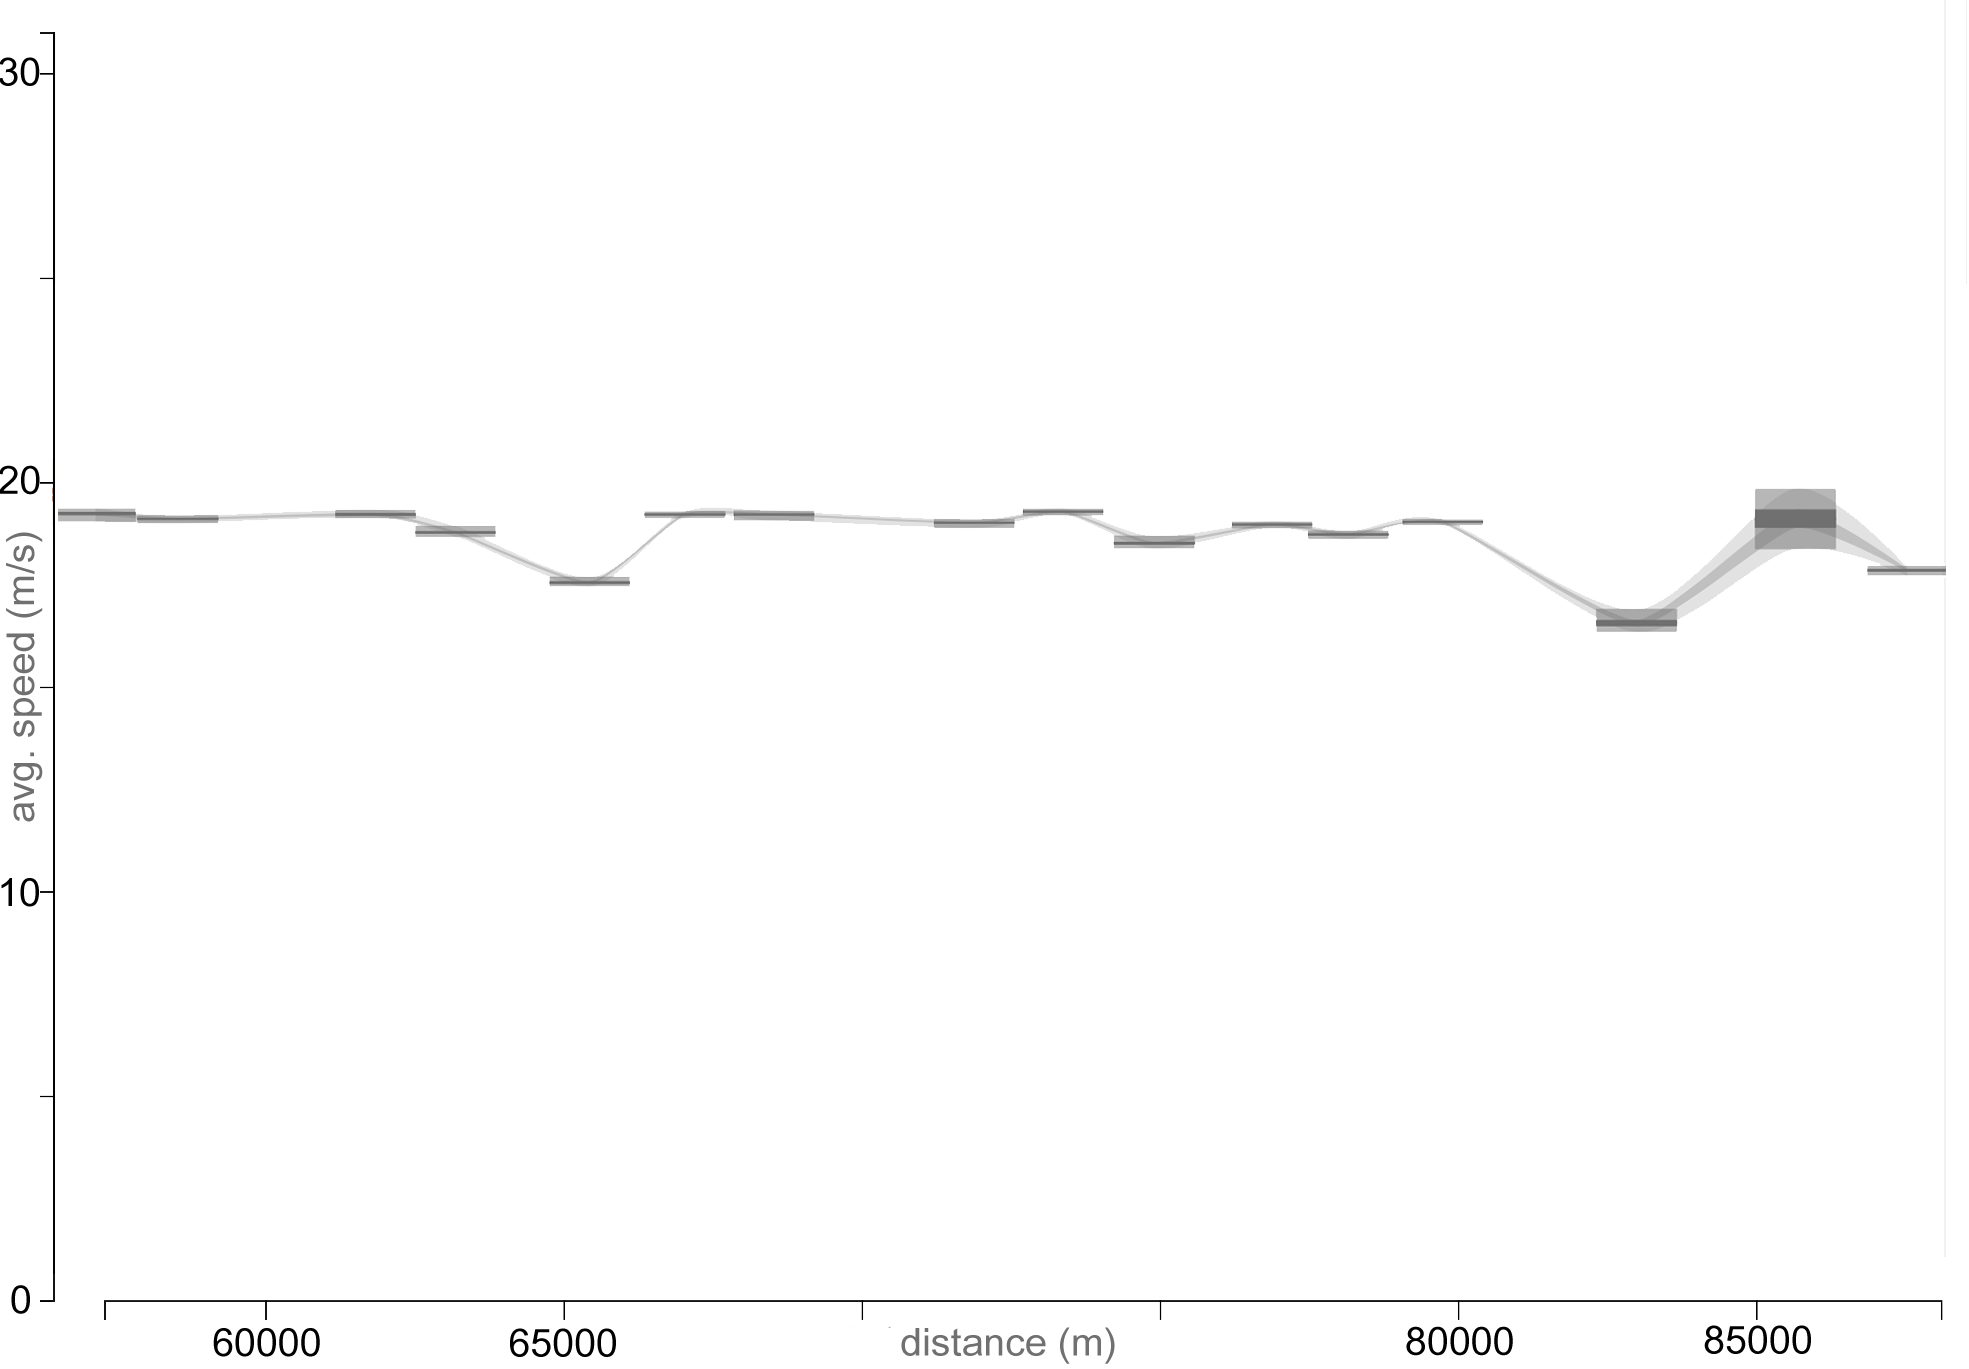
\includegraphics[width=\textwidth]{images/sampling/timestep_a_truth.png}
        \caption{Time window 1.}
        \label{fig:d}
    \end{subfigure}
    \begin{subfigure}{0.32\textwidth}
        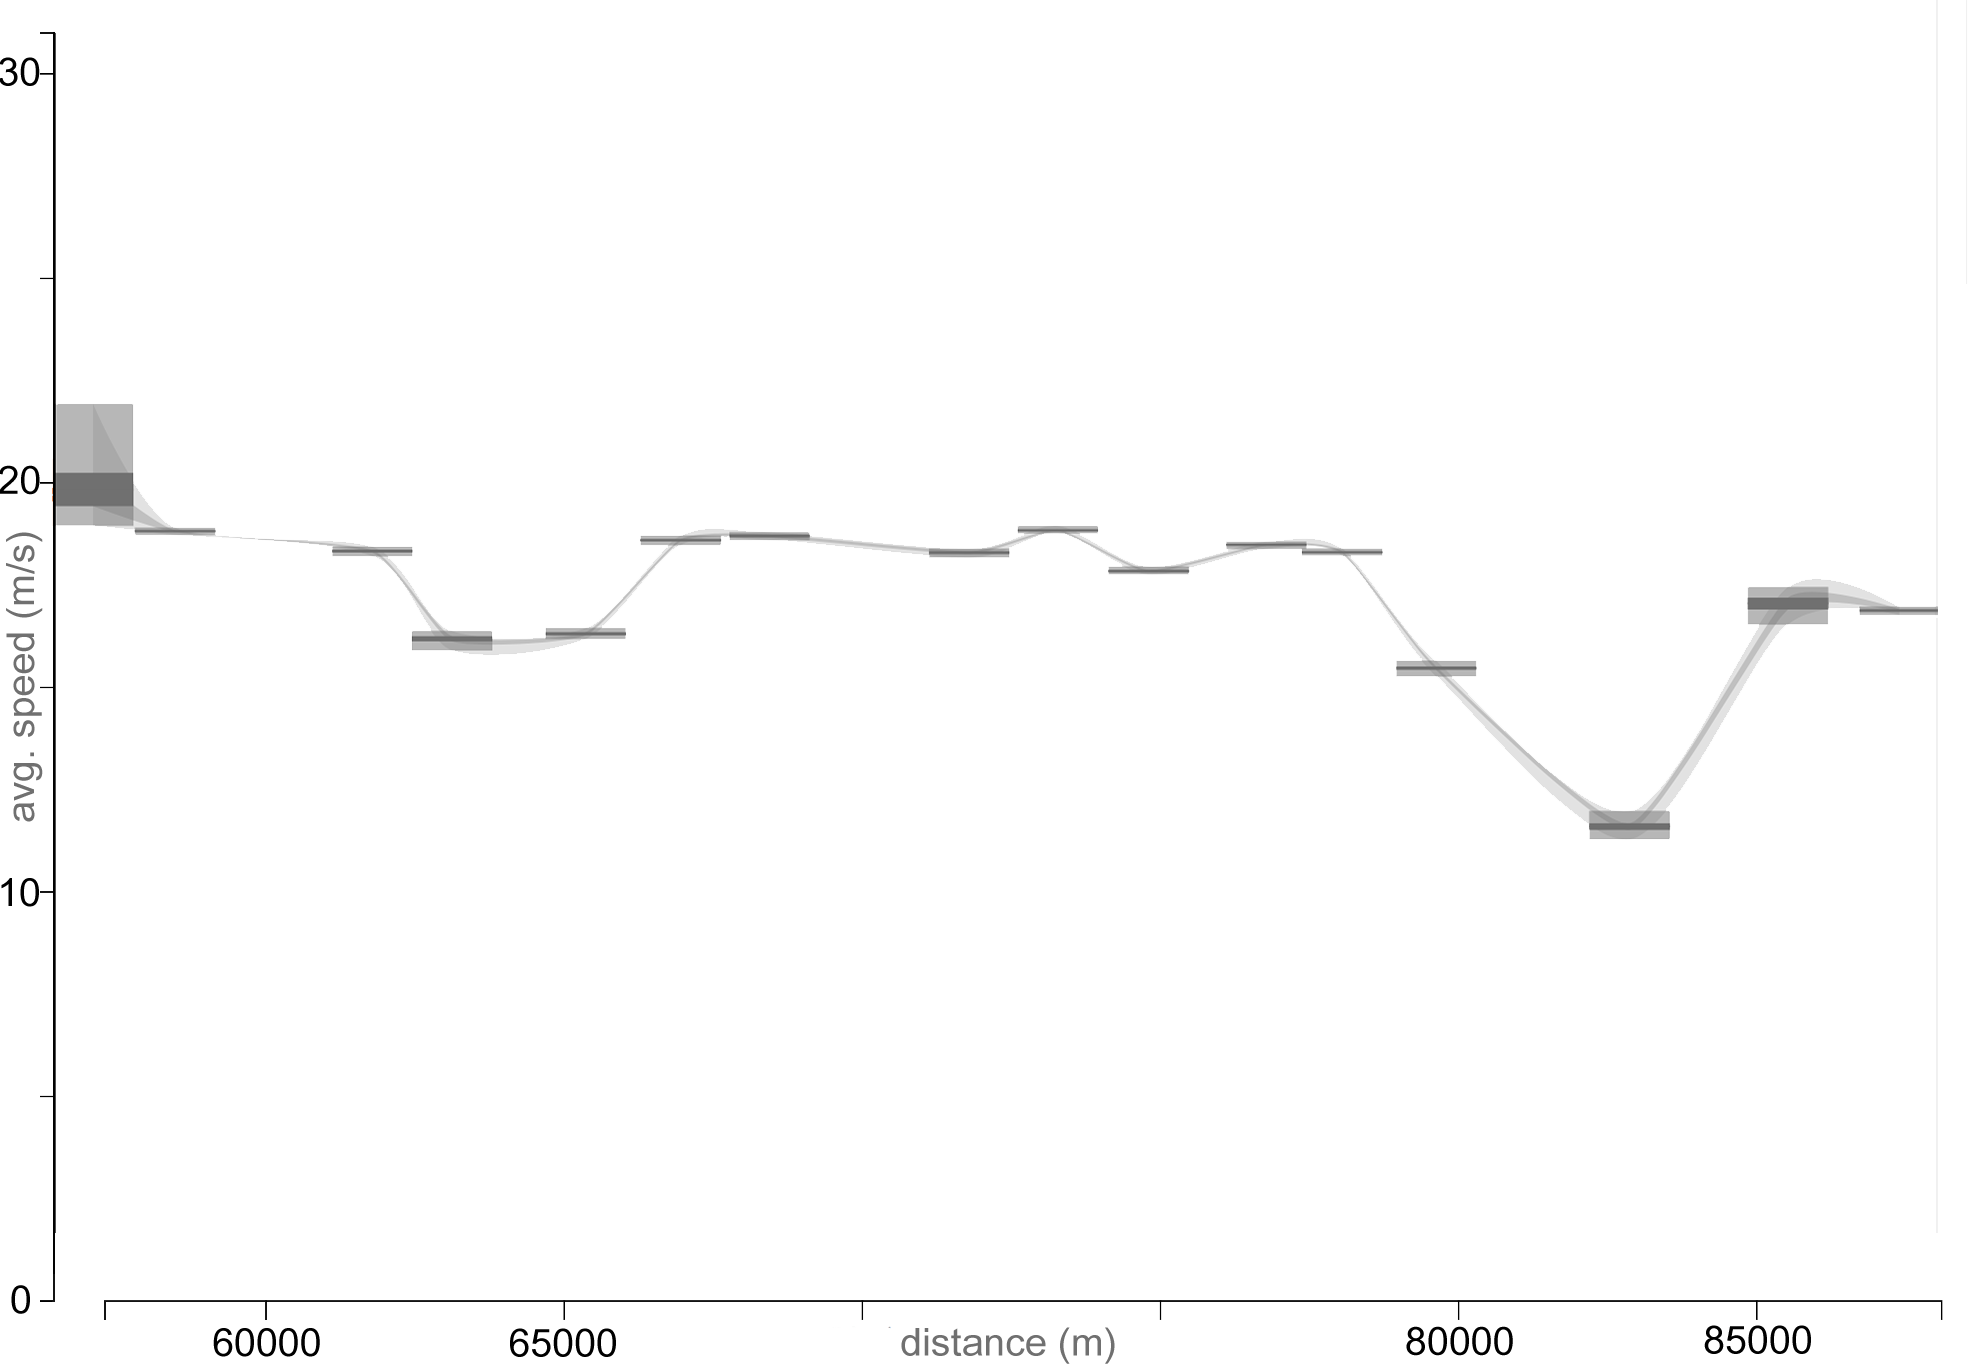
\includegraphics[width=\textwidth]{images/sampling/timestep_b_truth.png}
        \caption{Time window 2.}
        \label{fig:e}
    \end{subfigure}
    \begin{subfigure}{0.32\textwidth}
        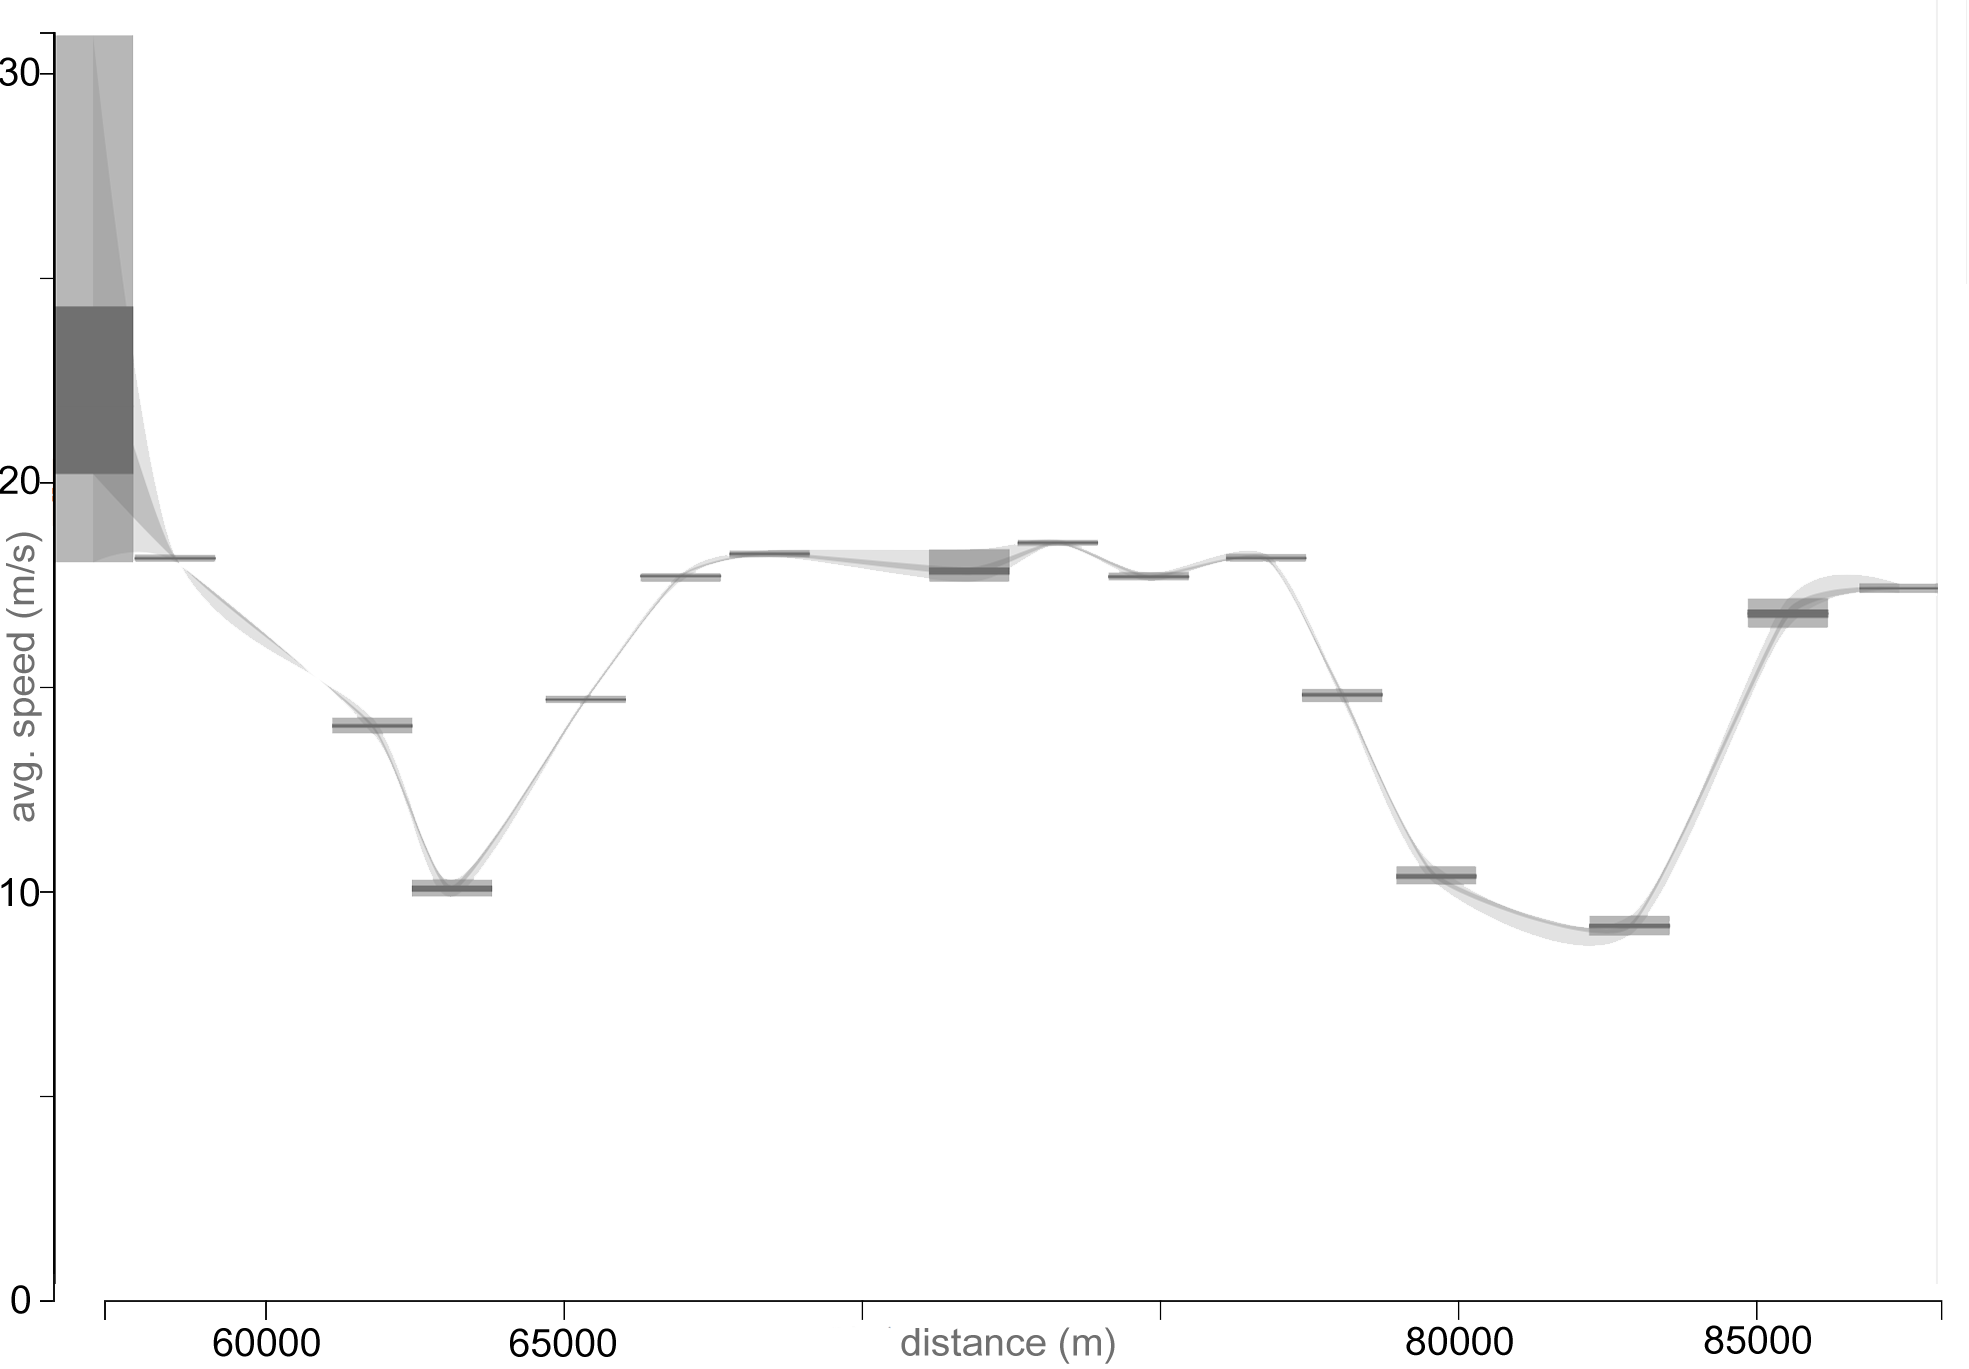
\includegraphics[width=\textwidth]{images/sampling/timestep_c_ground_truth.png}
        \caption{Time window 3.}
        \label{fig:f}
    \end{subfigure}
     \caption{The ``true'' variance in speed for the above scenario, calculated by bootstrapping over the full dataset for each time window.}
     \label{traffic}
\end{figure*}

\subsubsection{Analytical Needs}
The researchers confirmed that, in general, they are interested in ``teasing apart the sources of uncertainty,'' which may or may not be feasible. Lacking that information, they may present their results as a range of possible outcomes with associated confidences.

We proposed that our tool could enable both rapid, rougher estimates of uncertainty, as well as the option to further optimize the predictions. Somewhat surprisingly, there was especially strong interest in the first of these capabilities, the rougher, faster estimate.

One researcher specified that the precise optimization would be useful, but less useful than the less precise but more rapid prediction. He elaborated that at one point, there was a push within the climate modeling community to use ``adjoint methods'' (i.e., sensitivity analysis) to measure uncertainty, but they are quite expensive. “For instance, determining model sensitivity to the choice of particular tuning parameters typically requires 3-4 multi-decadal simulations to see the effect. This is generally untenable with limited computational resources.” Therefore, he said, our rapid estimation would be useful. This could allow scientists to determine which areas---time spans, sets of parameters, etc.---to measure more fully.

Another researcher added that ``basic quality checks are always important'' when analyzing simulations. Visualization to enable qualitative checks such as the growth of uncertainty over time would be very useful, because errors are likely to occur somewhere in the simulation or analysis codes, and visualization tools like ours could help perform basic ``sanity checks'' throughout the modeling process.

\begin{table}[h]
\caption {Training times, and sizes of samples used, for each dataset.} \label{speedup_table} 
\centering
\begin{tabular}{ >{\centering\arraybackslash}m{1.6in}  >{\centering\arraybackslash}m{1.5in} >{\centering\arraybackslash}m{1in} >{\centering\arraybackslash}m{0.5in} >{\centering\arraybackslash}m{1in} >{\centering\arraybackslash}m{1in}}
%\toprule[1.5pt]
%NOTE: edit fractions used based on final results.
{\bf Source} & {\bf Fractions Used} & {\bf Full Size} & {\bf Training}\\ 
Illustris (dark matter simulation) & 0.001, 0.002, 0.003, 0.005, 0.01  & 94 million particles & 188 s\\
\midrule
SUMO (traffic simulation) & 0.05, 0.1 & 9 million entries & 88 s\\
\midrule
CMIP5 (climate models) &  0.0001, 0.0002, 0.0005, 0.001, 0.002, 0.005 & $\sim$2GB per model & 110 s\\
%\bottomrule[1.25pt]
\end {tabular}
\end {table}

%(LK:) the precision needed is driven by what particular question you’re asking. he mentioned being more interested in ‘dominant’ sources of uncertainty. what conclusions are you trying to draw? once we understand a more dominant source of uncertainty, a smaller source of uncertainty may then become more interesting.

One of the atmospheric scientists shared his research interests in depth. He is interested in the likelihoods of extreme weather events, such as extreme precipitation, and how parameter choice affects these likelihoods. One needs many, very high-resolution model runs to properly characterize uncertainty, especially to capture unlikely events. He explores a seven-dimensional space of physical parameters, running a large ensemble of models with values that span the parameter space to try to figure out which sets of parameters most reflect reality. This approach is very expensive, and it is difficult to be sure that one is covering a representative sample of the parameter space, especially because results might not have a continuous dependence on a parameter or combination of parameters. 

%(BT: comparing likelihoods in different climate scenarios, e.g. human emissions and no human emissions. observations can be really hard to come by — only have good observational data for the world (with humans!) for last 30-50 years at best, and for the non-human data, have to be more resourceful (e.g. paleoclimatology?), so correctly characterizing the uncertainty in simulations is even more important

%(BT: talked about work that would have a similar workflow to his, with different particular parameters/outcomes being studied; really into the idea of a flexible tool that could accommodate all of tehse things. could use a list of standardized metrics of climate models that’s avaialble.

All of the researchers, whether working with observations or simulations, strongly emphasized the importance of understanding uncertainty as they work with ensembles of model outputs, and referred to the current difficulty of quantifying and comparing model uncertainties. 
They all assess uncertainty resulting from various parameter or input combinations regularly in their research.

%The workflow of assessing uncertainty resulting from various parameter combinations or initial conditions was common to all of the researchers.

\subsubsection{Our Approach}
The researchers we talked to felt confident that our method and visualization tool could provide useful and accurate information: ``the general idea of taking sub-samples...to inform what the uncertainty is of the ensemble, that's a very straightforward approach, which makes sense to me,'' one said. One person was particularly interested in being able to see the trends in all the samples. Several appreciated the idea that someone interacting with the tool would not have to worry about the specifics of the modeling behind-the-scenes.

Another researcher, the one who explores parameter spaces in climate models, was excited by the idea of an interface like ours, that one can plug any data into, adjust as needed, and flexibly see a quick result. He could imagine interactively tuning the parameters and getting a quick idea of how uncertainty varies with various combinations of parameters, showing him which parts of the parameter space to explore further; this could save a lot of time. We discussed the need for flexibility of data formats and parameter types; he felt it was reasonable for a tool to require a little bit of custom scripting for a particular use case. He pointed us to a standardized list of climate model measures, which could be built into our tool.

\subsection{Case Studies}
\label{results}
For each application---the SUMO traffic model; the Illustris dark matter simulation; the ensemble of CMIP5 ocean models---we show an example use of our method and visualization tool, and discuss successes and difficulties that are particular to each. To interpret the figures: in a boxplot representation, a smaller range indicates higher confidence, and the most likely outcomes are within the darker segments. Throughout this section, ``ground truth'' refers to the uncertainty measured by bootstrapping the full datasets until the results converge. Though we use the ground truth for validation, in a real-world scenario, we expect that users do not have access to the result of this time-consuming calculation.

\subsubsection{Case Study 1: Dark Matter Halos}
We demonstrate our method on halo mass functions in Figure~\ref{hmf_predicted}. In this case,  the halo masses scale with the size of the sample. Therefore, both the magnitudes and the relative values of the uncertainties are strongly dependent on sample size, and both relationships must be described in the model. Our results show a prediction of uncertainty that smoothly decreases with each mass bin, which is the behavior that the ground truth variance converges to.

The magnitude of variance in our prediction roughly matches the ground truth measurement. The predicted variance is on the order of $10^{-4} \mathrm{Mpc}^{-3}$, while the halo mass function peak is about $0.3\mathrm{Mpc}^{-3}$; this is within the desired precision of 1-5 percent~\cite{behroozi},~\cite{tinker}. 

A researcher could use a trained model to quickly check new simulation runs and determine whether the particle shot noise is likely to be within an acceptable level. In the case depicted in Figure~\ref{hmf_predicted}, he would decide that the simulation could proceed because the uncertainty meets the requirements for comparing simulation output to observed data. However, if the particle noise were projected to be too large, he could choose to stop this simulation run and investigate the problem before using more computing resources.

\subsubsection{Case Study 2: Traffic Jam Evolution}
We tested our approach on three consecutive time windows of the traffic model SUMO~\cite{SUMO2012} (see Section~\ref{traffic_sims}). Within each time window, we display the average speed of cars that pass several detectors, measured with two small samples of the simulation data. We simultaneously show the predicted uncertainty values (Figure~\ref{traffic_predicted}), and compare with our calculation of the ``true'' uncertainty (Figure~\ref{traffic}).  

In time window 1 (Figure~\ref{fig:d}), cars travel at a fairly consistent speed, with one slow-down around $x_a = 65,000$ and another, more significant, slow-down around $x_b = 80,000$. Imagine an emergency manager monitoring an evacuation route represented by this traffic model (Section~\ref{traffic_sims}). Looking at Figure~\ref{traffic}, she sees a confident prediction that the jam at $x_a$ will be alleviated after a short distance. 

Meanwhile, the emergency manager can see that for the jam at $x_b$, there is a much more significant probability that the jam will get worse through $x=83,000$m. Therefore, she focuses on this second jam location to look for alternate routes there. Indeed, in Figure 7 we see with high confidence that the second jam continues to worsen.

In general, our model overestimates the magnitude of the variance. Since the training samples display more variance in average speed (because outliers have a stronger influence over the average of smaller samples), this extra variance is reflected in our prediction. To mitigate this effect, one could include more samples; then, the model would have more training to recognize a diminishing variance with larger sample sizes. We see this in Figure~\ref{traffic_predicted}, where larger samples (orange) have slightly lower variance than smaller samples (green).

\label{ohc_case_study}
\begin{figure*}[h]
    \centering
    \begin{subfigure}{0.49\textwidth}
        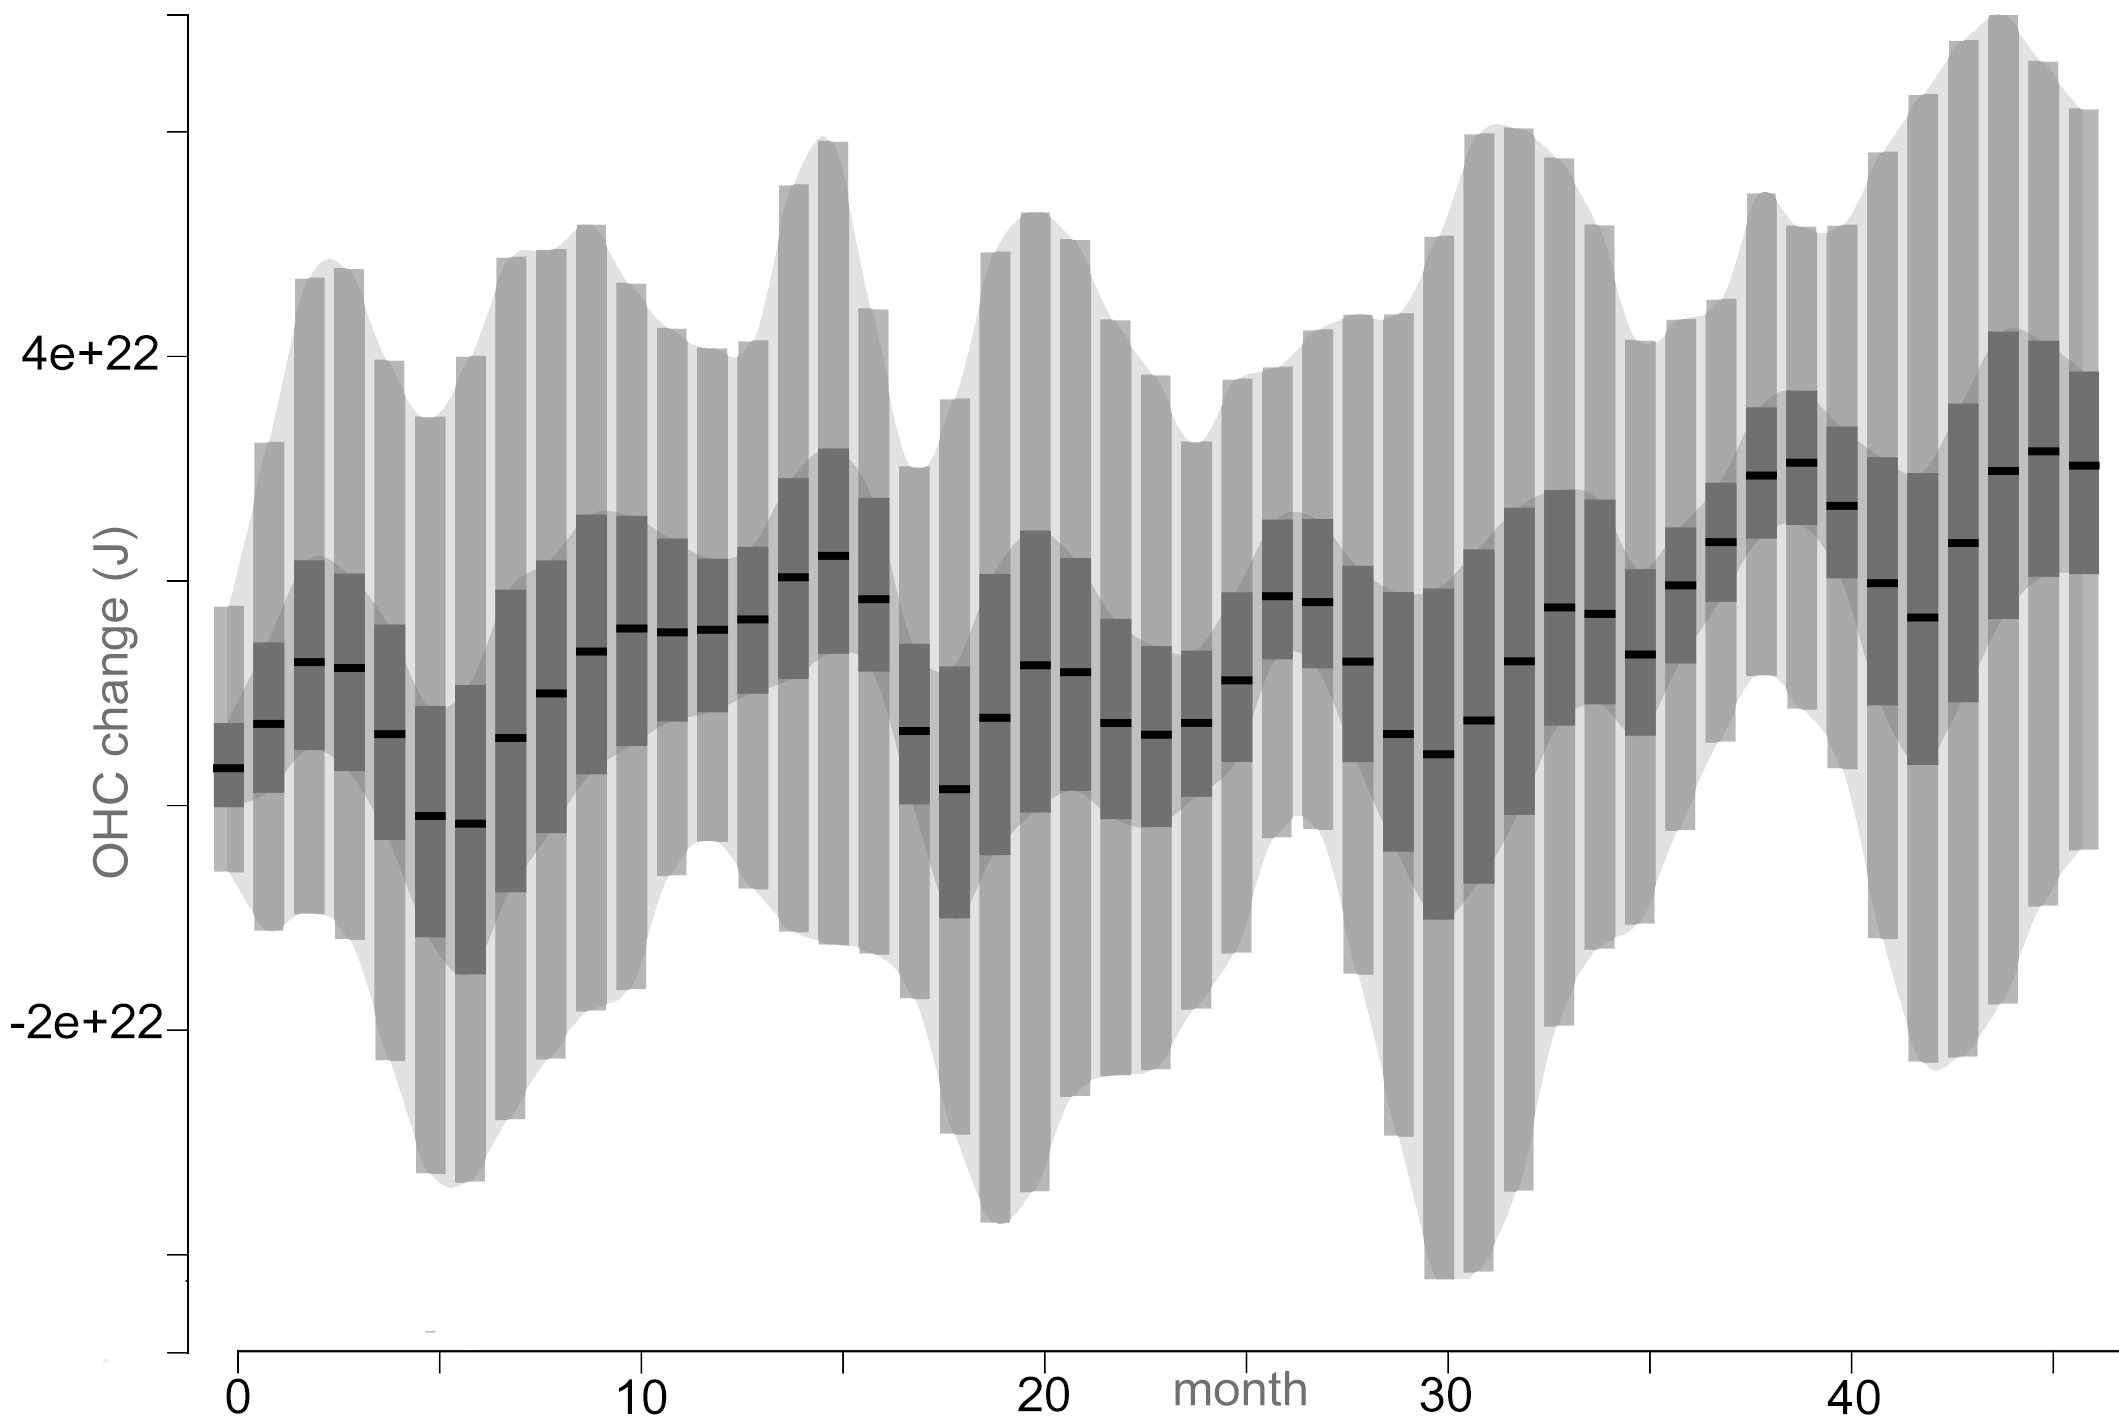
\includegraphics[width=\textwidth]{images/sampling/cmip_prediction_2006_2010_cropped.png}
        \caption{Predicted variance in ocean heat content change, 2006-2009.}
        \label{ohc_predicted_a}
    \end{subfigure}
    \begin{subfigure}{0.49\textwidth}
        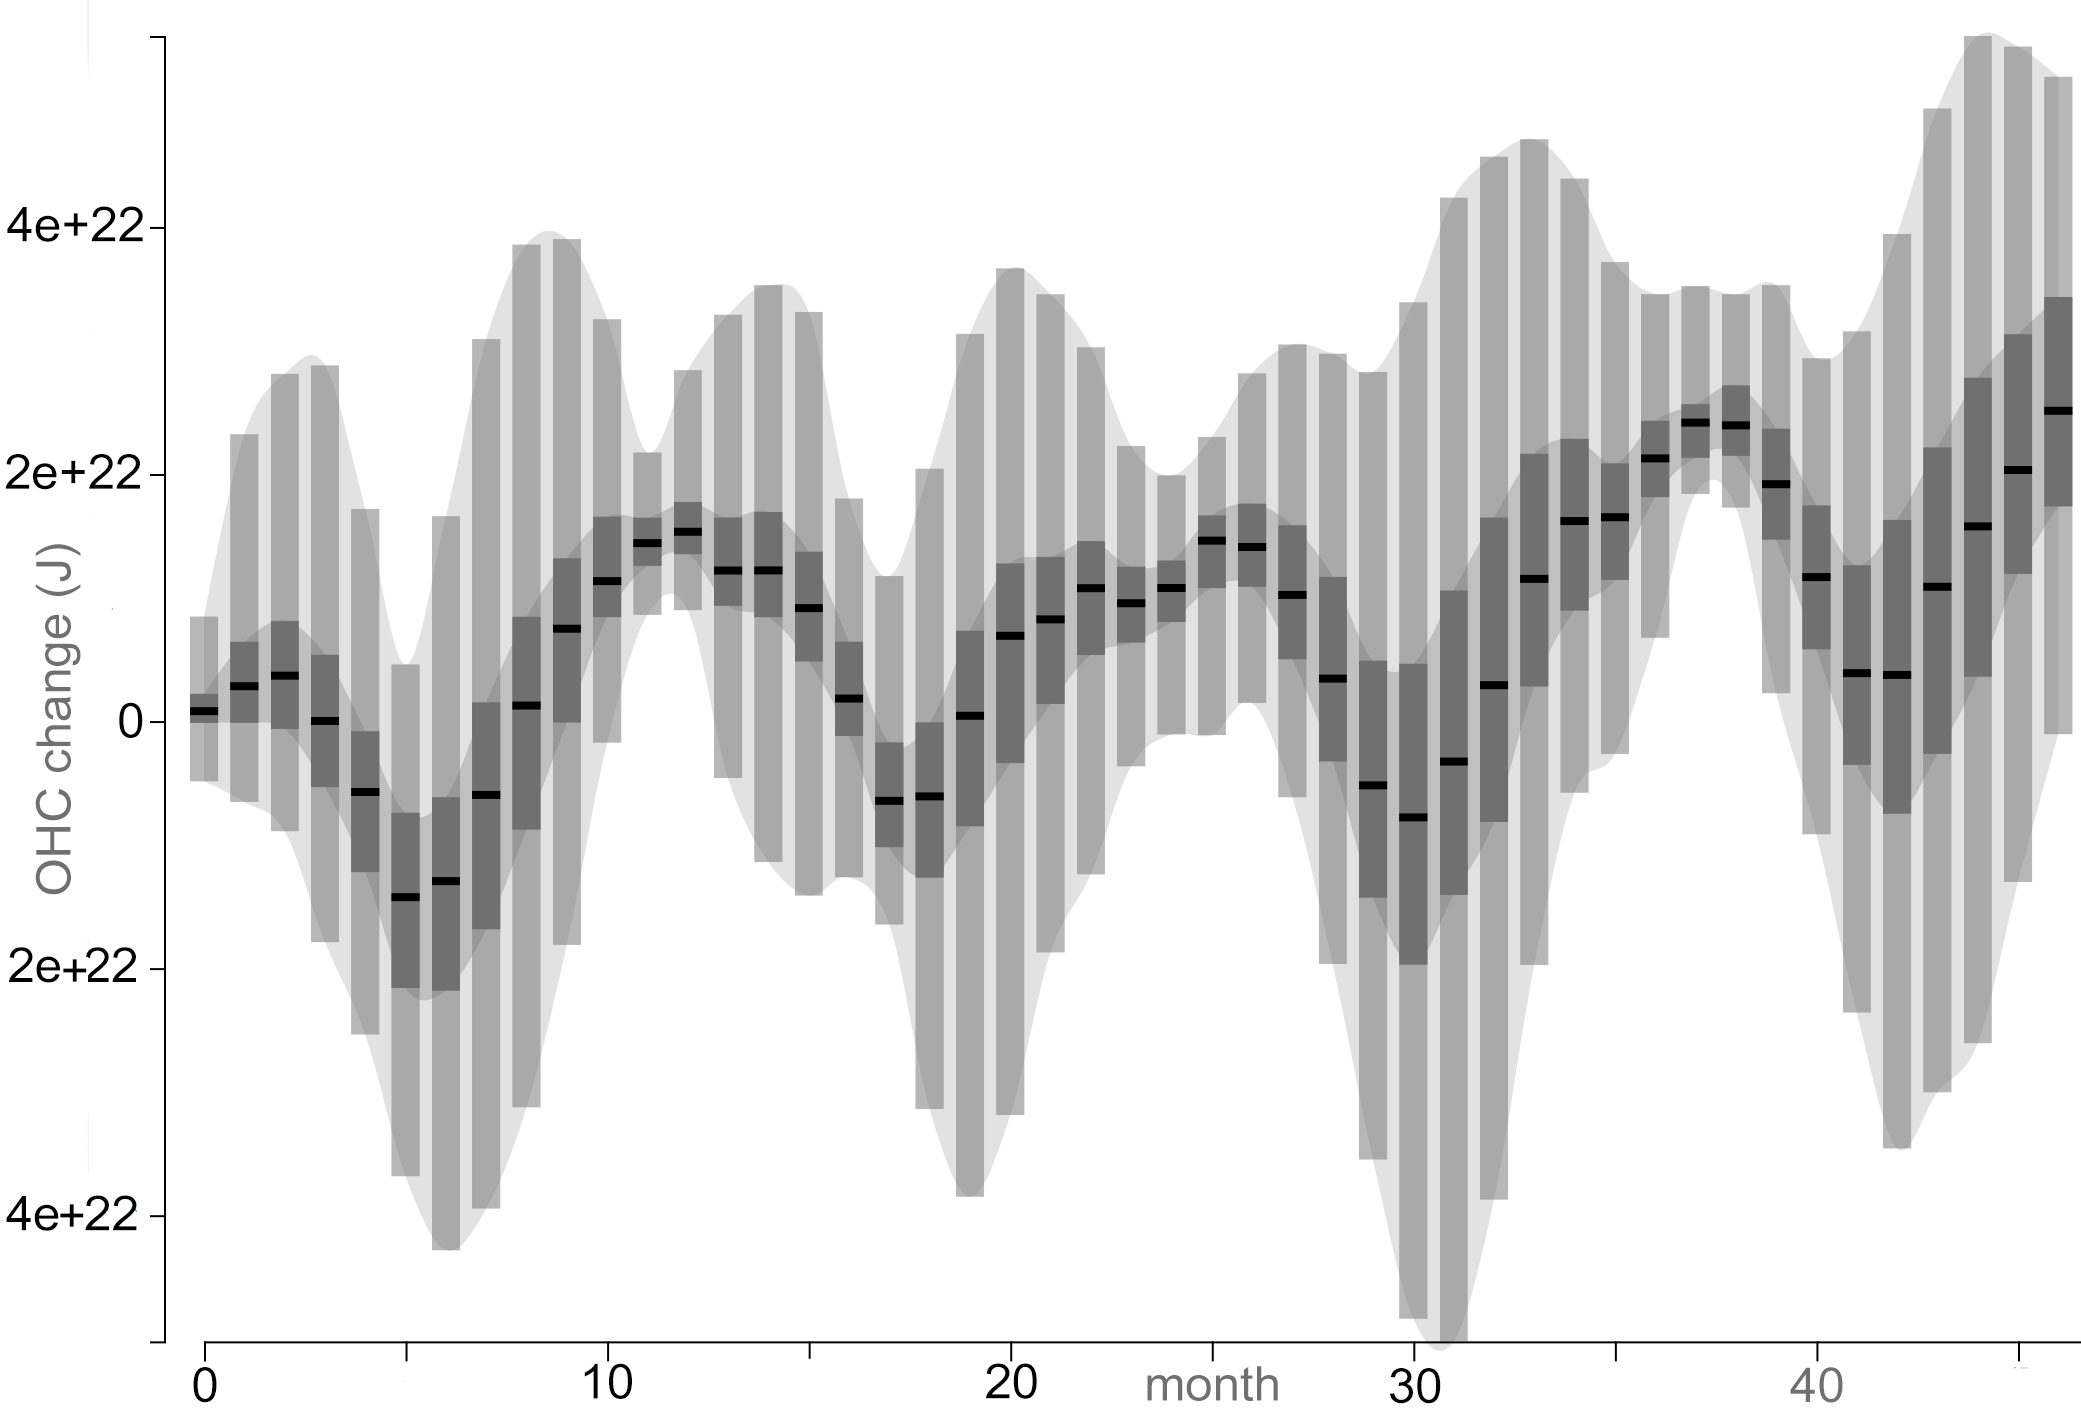
\includegraphics[width=\textwidth]{images/sampling/cmip_ground_truth_2006_2010.png}
        \caption{``True'' variance in ocean heat content change, 2006-2009.}
        \label{ohc_true_a}
    \end{subfigure}
     \caption{CMIP5 ensemble data from 2006-2009.}
     \label{ohc_a}
\end{figure*}

\begin{figure*}[h]
    \centering
    \begin{subfigure}{0.49\textwidth}
         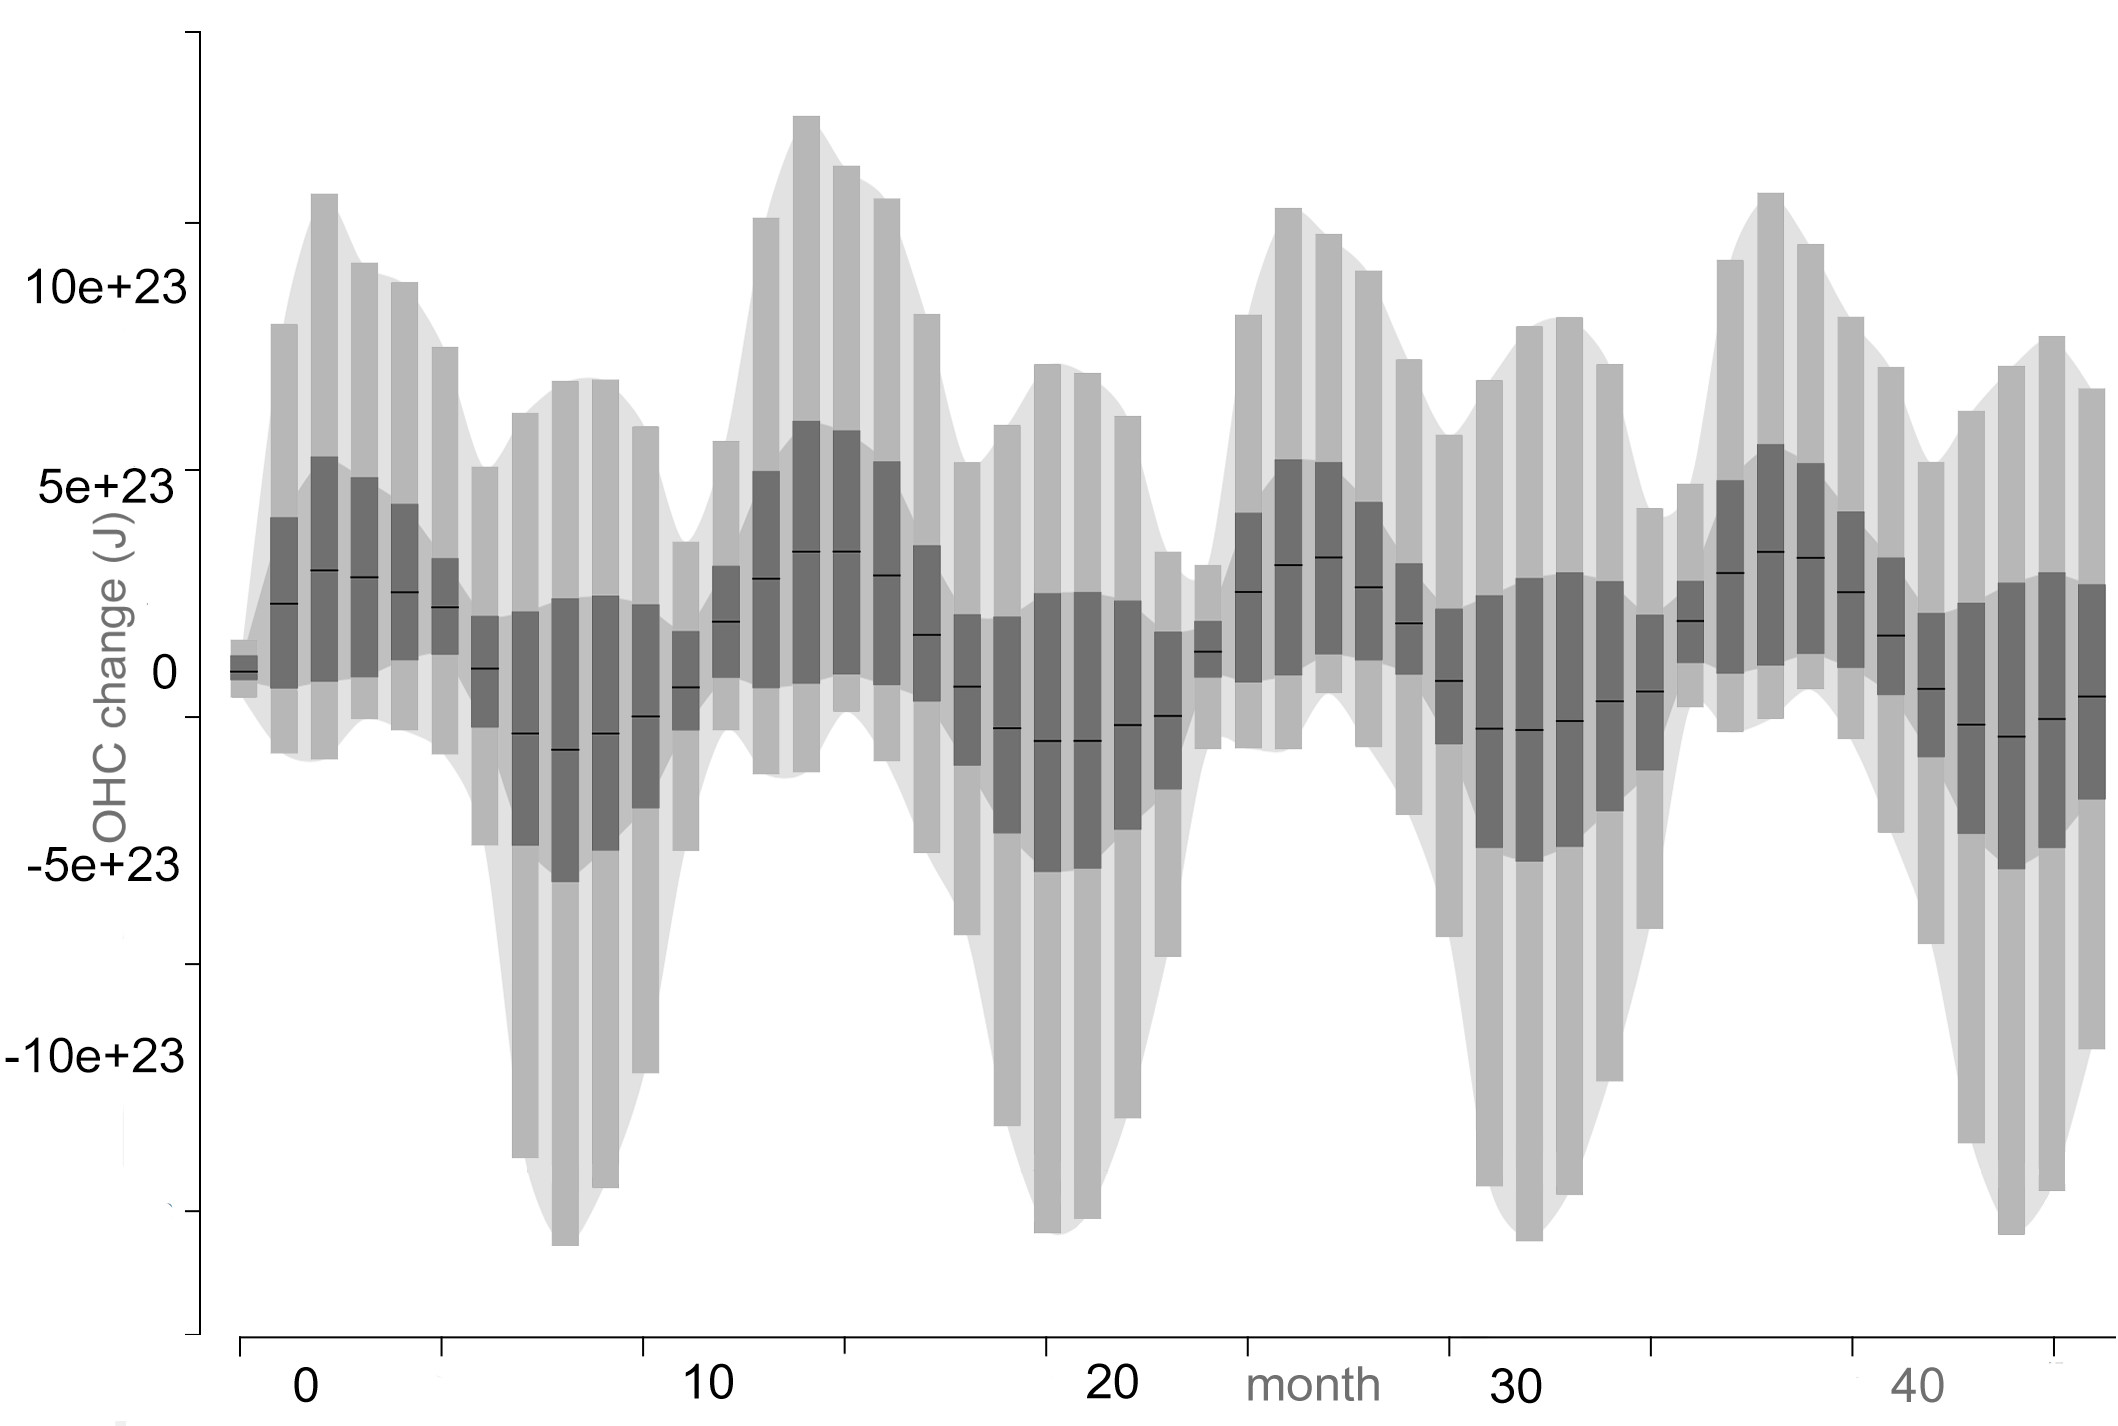
\includegraphics[width=\textwidth]{images/sampling/2010_2014_predictions}
        \caption{Variance in ocean heat content change, predicted with the model trained above (Figure~\ref{ohc_predicted_a}), 2010-2013.}
        \label{ohc_predicted_b}
    \end{subfigure}
    \begin{subfigure}{0.49\textwidth}
        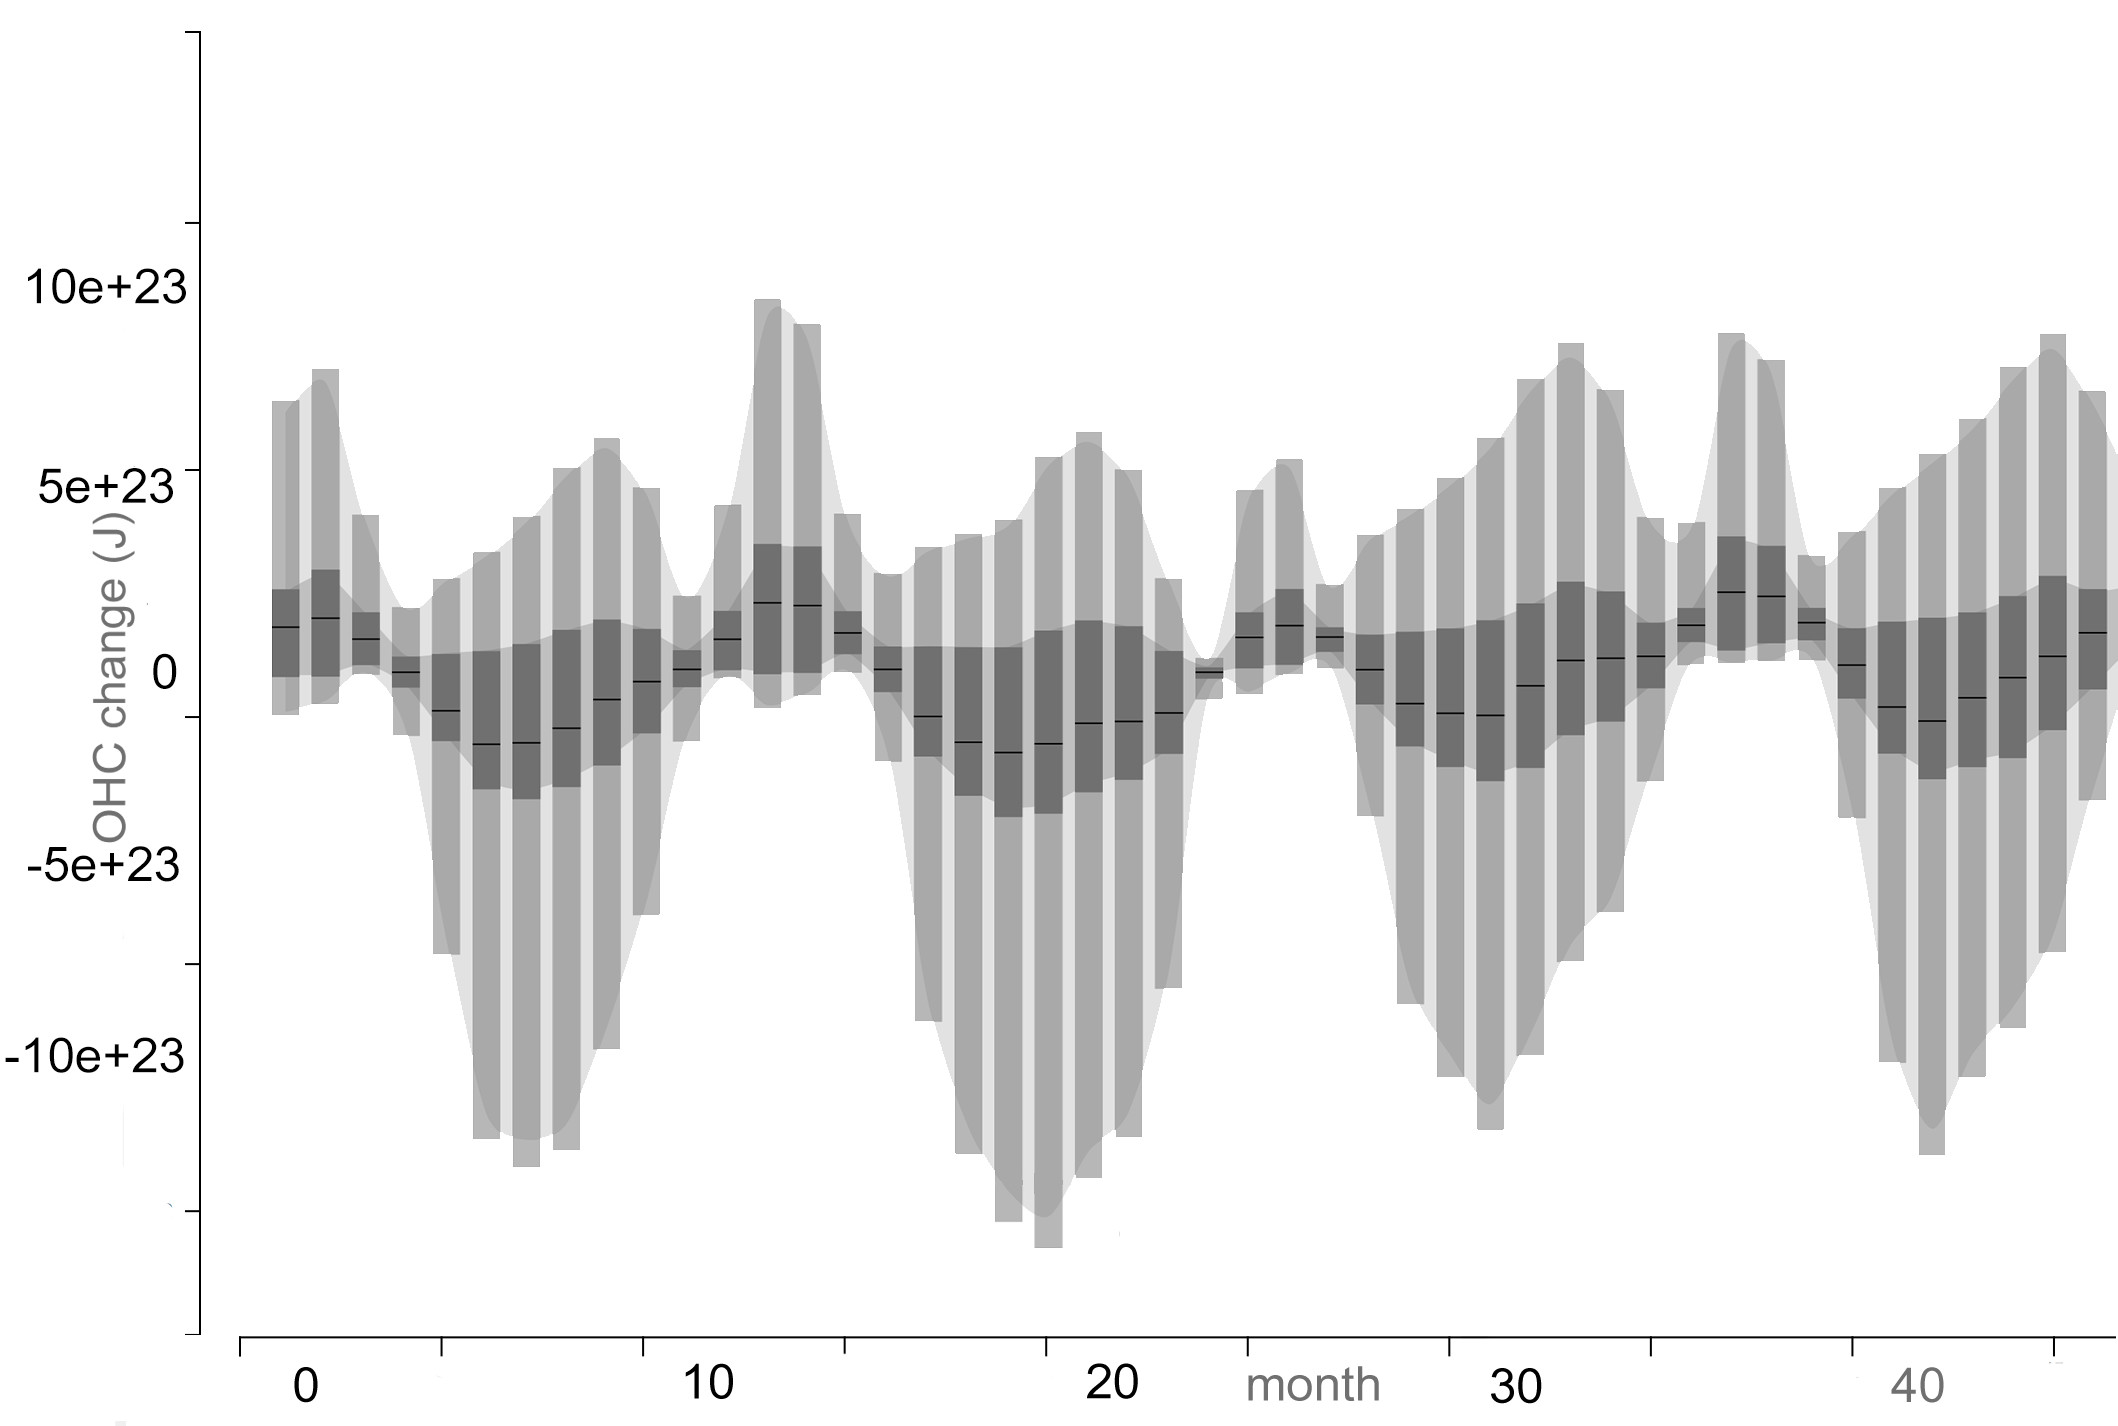
\includegraphics[width=\textwidth]{images/sampling/cmip_truth_2010-2014}
        \caption{True variance in ocean heat content change, 2010-2013.}
        \label{ohc_true_b}
    \end{subfigure}
     \caption{CMIP5 ensemble data from 2010-2013 (a different combination of models than those used in training), the testing dataset.}
     \label{ohc_b}
\end{figure*}

\subsubsection{Case Study 3: Rising Ocean Heat Content}
As described in Section~\ref{climate_models}, we sampled an ensemble of ocean models, then performed our bootstrapping method over the ensemble to measure uncertainty. Our set of models is smaller than ensembles that researchers may use in practice, so our results are noisier than real-world results might be. The shape of the uncertainty contours is largely accurate: almost all of the values have the correct relationships with neighboring values, and the periodic increase is reflected. However, our model (Figures~\ref{ohc_predicted_a},~\ref{ohc_predicted_b}) overestimates the magnitude of the variance (Figures~\ref{ohc_true_a},~\ref{ohc_true_b}). In general, scientists are interested in constraining uncertainty; overestimation can still be useful. 

Many scientists are primarily interested in the relative confidence levels for different sets of parameters. A researcher could use our prediction to see that, for the set of parameters used in our example, the magnitude of uncertainty tends to increase at later times, and that the peak OHC values (e.g. month 26, month 38) have higher confidence than the lower values. Then, the researcher could feed another dataset to the model, such as a sample from another simulation with different input parameters or initial conditions, to see how this difference affects the confidence in the OHC values. We tested this workflow by applying our trained model to OHC values from another ensemble of CMIP5 simulations for a different time period, 2010-2013 (see Figure~\ref{ohc_predicted_b}). The prediction shows a higher likelihood of greater seasonal swings in OHC than in the years 2006-2009. This increasingly volatile behavior is confirmed in Figure~\ref{ohc_true_b}.
	
The most accurate results we obtained for this case study omitted the three smallest sample sizes we had taken (see Table~\ref{speedup_table}). Comparing uncertainties for these samples in the interface, we could see that the smallest samples did not have a consistent pattern. Omitting these samples, we got a better prediction result; this is an example of how human-guided reasoning with our tool is a helpful supplement to modeling.
    %note: if/when i present about this, this would be a good example slide

% this phenomenon is something to watch out for when the measurement is an average (?). (Similar to climate.)

%explain the other outliers.

%quantitative results here.

\subsubsection{Performance}
%Results go here.
Compared to calculating uncertainty with bootstrapping on a full dataset, our method offers a speedup of $\mathcal{O}(N)$ (where $N$ represents the sample sizes used). That is, for each of our case studies, the relationship between sample size and uncertainty computation time is roughly linear. Note that, for the dark matter data, our speedup is highly dependent on halo finder implementation; some halo finders can be parallelized for efficient performance, though halo finding in general is quite expensive.

We also report model training times in MATLAB for each of the applications. These times were measured on an iMac with a 4GHz processor. Our aim is to show our method's feasibility with easily accessible computing resources. These times reflect the results shown in the case study images, but more precise results are usually possible with more fitting iterations and/or more hyperparameters.

% SHOW SCALABILITY.
%\caption {Training time for the regression model in each case study.}
%\label{speedup_table}

\subsection{Limitations}
%Lower limit on sample sizes.
For each application, there is a lower limit on the possible sample sizes. One reason is that a sufficiently small sample size captures too little information to provide to a model; these very small samples may omit large groups of outliers and/or be overly influenced by the inclusion of outliers (see section~\ref{traffic_case_study}). It should be possible, however, to identify these cases using our tool. If sampled uncertainties do not follow any discernible pattern, they are likely too subject to noise and therefore too small to use for modeling. With an increased simulation size, one can attain equally good results with smaller relative fractions; however, too extreme a discrepancy between sample size and absolute size makes extrapolation difficult.

% unsure whether this would work on all simulation types! e.g. astrophysical ones. depends on type of data and type of measurement, probably. future work can come up with more concrete limitations.

%scaling / log ...

% wrap up with summary of what works & what doesn't for each application we tested.
% - HMF was very hard because of the scaling; also, there are some pretty scalable halo finding algorithms out there, so it's harder for us to claim a significant improvement
% - OHC was easier, but ...
% - traffic ?

\section{Conclusion and Future Work}
Our method and visualization tool can facilitate fast estimates of discreteness uncertainty in several types of simulations. We establish that our method is generally transferable to researchers who need to characterize uncertainty in their simulations. However, in this study, we limit our tests to one category of uncertainty, which we measure with one type of approach. Separating sources of uncertainty is difficult, so our method provides the benefit of understanding one particular source in isolation. In the future, though, more tools need to be created, with capabilities such as sensitivity analysis to separate causes of uncertainty, and offering enhanced ability to supervise prediction kernels.

Methods and tools such as ours can be used as a basis to implement more complex or domain-specific uncertainty quantification. More broadly, tools like ours, which favor generalizability and applicability to realistic scenarios over precision, will be crucial for expanding the next generation of usable scientific visualization tools.